%!TEX TS-program = xelatex
% !TEX root = ../thesis.tex
% Do not delete; used to set build system

%\begin{savequote}[75mm] 
%Nulla facilisi. In vel sem. Morbi id urna in diam dignissim feugiat. Proin molestie tortor eu velit. Aliquam erat volutpat. Nullam ultrices, diam tempus vulputate egestas, eros pede varius leo.
%\qauthor{Quoteauthor Lastname} 
%\end{savequote}

\chapter{The promise and perils of preprocessing: building foundations for multiphase inference}
\label{multiphase:ch:multiphase}

\section{Summary}

Preprocessing forms an oft-neglected foundation for a wide range of statistical and scientific analyses.
However, it is rife with subtleties and pitfalls.
Decisions made in preprocessing constrain all later analyses and are typically irreversible.
Hence, data analysis becomes a collaborative endeavor by all parties involved in data collection, preprocessing and curation, and downstream inference.
Even if each party has done its best given the information and resources available to them, the final result may still fall short of the best possible in the traditional single-phase inference framework.
This is particularly relevant as we enter the era of ``big data''.
The technologies driving this data explosion are subject to complex new forms of measurement error.
Simultaneously, we are accumulating increasingly massive databases of scientific analyses.
As a result, preprocessing has become more vital (and potentially more dangerous) than ever before.

We propose a theoretical framework for the analysis of preprocessing under the banner of multiphase inference.
We provide some initial theoretical foundations for this area, including distributed preprocessing, building upon previous work in multiple imputation.
We motivate this foundation with two problems from biology and astrophysics, illustrating multiphase pitfalls and potential solutions.
These examples also emphasize the motivations behind multiphase analyses---both practical and theoretical.
We demonstrate that multiphase inferences can, in some cases, even surpass standard single-phase estimators in efficiency and robustness.
Our work suggests several rich paths for further research into the statistical principles underlying preprocessing.
%
%Our work highlights the importance of providing information beyond ``optimal''
%estimators for downstream analyses.
%
To tackle our increasingly complex and massive data, we must ensure that our inferences are built upon solid inputs and sound principles.
Principled investigation of preprocessing is thus a vital direction for statistical research.

\section{What is multiphase inference?}

\subsection{Defining multiphase problems}
Preprocessing and the analysis of preprocessed data are ubiquitous components of statistical analysis, but their treatment has often been informal.
We aim to develop a theory that provides a set of formal statistical principles for such problems under the banner of multiphase inference.
The term ``multiphase'' refers to settings in which inferences are obtained through the application of multiple procedures in sequence, with each procedure taking the output of the previous phase as its input.
This encompasses settings such as multiple imputation \citep[MI,][]{Rubin1987} and extends to other situations.
In a multiphase setting, information can be passed between phases in an arbitrary form; it need not consist of (independent) draws from a posterior predictive distribution, as is typical with multiple imputation.
Moreover, the analysis procedure for subsequent phases is not constrained to a particular recipe, such as Rubin's MI combining rules \citep{Rubin1987}.

The practice of multiphase inference is currently widespread in applied statistics.
It is widely used as an analysis technique within single publications---any paper that uses a ``pipeline'' to obtain its final inputs or clusters estimates from a previous analysis provides an example.
Furthermore, projects in astronomy, biology, ecology, and social sciences (to name a small sampling) increasingly focus on building databases for future analyses as a primary objective.
These projects must decide what levels of preprocessing to apply to their data and what additional information to provide to their users.
Providing all of the original data clearly allows the most flexibility in subsequent analyses.
In practice, the journey from raw data to a complete model is typically too intricate and problematic for the majority of users, who instead choose to use preprocessed output.

Unfortunately, decisions made at this stage can be  quite treacherous. Preprocessing is typically irreversible, necessitating assumptions about both the observation mechanisms and future analyses. These assumptions constrain all subsequent analyses.
Consequently, improper processing can cause a disproportionate amount of damage to a whole body of statistical results.
However, preprocessing can be a powerful tool.
It alleviates complexity for downstream researchers, allowing them to deal with smaller inputs and (hopefully) less intricate models.
This can provide large mental and computational savings.

Two examples of such trade-offs come from NASA and high-throughput biology.
When NASA satellites collect readings, the raw data are usually massive.
These raw data are referred to as the ``Level 0'' data \citep{ChandraSDP}.
The Level 0 data are rarely used directly for scientific analyses.
Instead, they are processed to Levels 1, 2, and 3, each of which involves a greater degree of reduction and adjustment.
Level 2 is typically the point at which the processing becomes irreversible.
\cite{Braverman2012} provide an excellent illustration of this process for the Atmospheric Infrared Sounder (AIRS) experiment.
This processing can be quite controversial within the astronomical community.
Several upcoming projects, such as the Advanced Technology Solar Telescope (ATST) will not be able to retain the Level 0 or Level 1 data \citep{Davey2012}.
This inability to obtain raw data and increased dependence on preprocessing has transformed low-level technical issues of calibration and reduction into a pressing concern.

High-throughput biology faces similar challenges.
Whereas reproducibility is much needed \citep[e.g.,][]{Ioannidis2011}, sharing raw datasets is difficult because of their sizes.
The situation within each analysis is similar.
Confronted with an overwhelming onslaught of raw data, extensive preprocessing has become crucial and ubiquitous.
Complex models for genomic, proteomic, and transcriptomic data are usually built upon these heavily-processed inputs.
This has made the intricate details of observation models and the corresponding preprocessing steps the groundwork for entire fields.

To many statisticians, this setting presents something of a conundrum.
After all, the ideal inference and prediction will generally use a complete correctly-specified model encompassing the underlying process of interest and all observation processes.
Then, why are we interested in multiphase?
We focus on settings where there is a natural separation of knowledge between analysts, which translates into a separation of effort.
The first analyst(s) involved in preprocessing often have better knowledge of the observation model than those performing subsequent analyses.
For example, the first analyst may have detailed knowledge of the structure of experimental errors, the equipment used, or the particulars of various protocols.
This knowledge may not be easy to encapsulate for later analysts---the relevant information may be too large or complex, or the methods required to exploit this information in subsequent analyses may be prohibitively intricate.
%
% As mentioned previously, such cases are ubiquitous across many scientific fields.
%
Hence, the practical objective in such settings is to enable the best possible inference given the constraints imposed and provide an account of the trade-offs and dangers involved.
To borrow the phrasing of \citet{Meng2003} and \citet{Rubin1996}, we aim for achievable practical efficiency rather than a theoretical efficiency that is practically unattainable.

Multiphase inference currently represents a serious gap between statistical theory and practice.
We typically delineate between the informal work of preprocessing and feature engineering and formal, theoretically-motivated work of estimation, testing, and so forth.
However, the former fundamentally constrains what the latter can accomplish.
As a result, we believe that it represents a great challenge and opportunity to build new statistical foundations to inform statistical practice.

\subsection{Practical motivations}
\label{multiphase:sec:examples}

We present two examples  that show both the impetus for and perils of undertaking multiphase analyses in place of inference with a complete, joint model. The first concerns  microarrays,  which allow the analysis of thousands of genes in parallel.
We focus on expression microarrays, which measure the level of gene expression in populations of cells based upon the concentration of RNA from different genes.
These are typically used to study changes in gene expression between different experimental conditions.

In such studies, the estimand of interest is typically the log-fold change in gene expression between conditions.
However, the raw data consist only of intensity measurements for each probe on the array, which are grouped by gene along with some form of controls.
These intensities are subject to several forms of observation noise, including additive background variation and additional forms of interprobe and interchip variation (typically modeled as multiplicative noise).
To deal with these forms of observation noise, a wide range of background correction and normalization strategies have been developed \citep[for a sampling, see][]{Tusher2001,Quackenbush2002,Affymetrix2002,Irizarry2003,McGee2006,Ritchie2007,Xie2009}.
Later analyses then focus on the scientific question of interest without, for the most part, addressing the underlying details of the observation mechanisms.

Background correction is a particularly crucial step in this process, as it is typically the point at which the analysis moves from the original intensity scale to the log-transformed scale.
As a result, it can have a large effect on subsequent inferences about log-fold changes, especially for genes with low expression levels in one condition \citep{Smyth2005,Irizarry2006}.
One common method (MAS5),  provided by one microarray manufacturer, uses a combination of background subtraction and truncation at a fixed lower threshold for this task \citep{Affymetrix2002}. Other more sophisticated techniques use explicit probability models for this de-convolution.
A model with normally-distributed background variation and exponentially distributed expression levels has proven to be the most popular in this field \citep{McGee2006,Xie2009}.

Unfortunately, even the most sophisticated available techniques pass only point estimates onto downstream analyses.
This necessitates ad-hoc screening and corrections in subsequent analyses, especially when searching for significant changes in expression \citep[e.g.,][]{Tusher2001}.
Retaining more information from the preprocessing phases of these analyses would allow for better, simpler inference techniques with greater power and fewer hacks.
The motivation behind the current approach is quite understandable: scientific investigators want to focus on their processes of interest without becoming entangled in the low-level details of observation mechanisms.
Nevertheless, this separation can clearly compromise the validity of their results.

The role of preprocessing in microarray studies extends well beyond background correction.
Normalization of expression levels across arrays, screening for data corruption, and other transformations preceding formal analysis are standard.
Each technique can dramatically affect downstream analyses.
For instance, quantile normalization equates quantiles of expression distributions between arrays, removing a considerable amount of information.
This mutes systematic errors \citep{Bolstad2003}, but it can seriously compromise analyses in certain contexts (e.g., miRNA studies).

Another example of multiphase inference can be found in the estimation of correlations based upon indirect measurements.
This appears in many fields, but astrophysics provides one recent and striking case.
The relationships between the dust's density, spectral properties, and temperature are of interest in studies of star-forming dust clouds.
These characteristics shed light on the mechanisms underlying star formation and other astronomical processes.
Several studies \citep[e.g.,][]{Dupac2003,Desert2008,Anderson2010,Paradis2010} have investigated these relationships, finding negative correlations between the dust's temperature and spectral index.
This finding is counter to previous astrophysical theory, but it has generated  many alternative explanations.

Such investigations may, however, be chasing a phantasm.
These correlations have been estimated by simply correlating point estimates of the relevant quantities (temperature $T$ and spectral index $\beta$) based on a single set of underlying observations.
As a result, they may conflate properties of this estimation procedure with the underlying physical mechanisms of interest.
This has been noted in the field by \citet{Shetty2009}, but the scientific debate on this topic continues.
\cite{Kelly2012} provide a particularly strong argument, using a cohesive hierarchical Bayesian approach, that improper multiphase analyses have been a pervasive issue in this setting.
Improper preprocessing led to incorrect, negative estimates of the correlation between temperature and spectral index, according to \cite{Kelly2012}.
These incorrect estimates even appeared statistically significant with narrow confidence intervals based on standard methods.
On a broader level, this case again demonstrates some of the dangers of multiphase analyses when they are not carried out properly.
Those analyzing this data followed an intuitive strategy: estimate what we want to work with ($T$ and $\beta$), then use it to estimate the relationship of interest.
Unfortunately, such intuition is not a recipe for valid statistical inference.%, as we shall demonstrate in this paper.

\subsection{Related work}

Multiphase inference has wide-ranging connections to both the theoretical and applied literatures.
It is intimately related to previous work on multiple imputation and missing data \citep{Rubin1976,Rubin1987,Meng1994,Rubin1996,Meng2003,Xie2012}.
In general, the problem of multiphase inference can be formulated as one of missing data.
However, in the multiphase setting, missingness arises from the preprocessing choices made, not a probabilistic response mechanism.
Thus, we can leverage the mathematical and computational methods of this literature, but many of its conceptual tools need to be modified.
Multiple imputation addresses many of the same issues as multiphase inference and is indeed a special case of the latter.
Concepts such as congeniality between imputation and analysis models and self-efficiency \citep{Meng1994} have natural analogues and roles to play in the analysis of multiphase inference problems.

Multiphase inference is also tightly connected to work on the comparison of experiments and approximate sufficiency, going back to \citet{Blackwell51,Blackwell53} and continuing through \citet{LeCam1964} and \citet{Goel79}, among others.
This literature has addressed the relationship between decision properties and the probabilistic structure of experiments, the relationship between different notions of statistical information, and notions of approximate sufficiency---all of these are quite relevant for the study of multiphase inference.
We view the multiphase setting as an extension of this work to address a broader range of real-world problems, as we will discuss in Section~\ref{multiphase:sec:riskmonotone}.

The literature on Bayesian combinations of experts also informs our thinking on multiphase procedures.
\citet{Kadane1993} provides an excellent review of the field, while \citet{Lindley1979} provides the core formalisms of interest for the multiphase setting.
Overall, this literature has focused on obtaining coherent (or otherwise favorable) decision rules when combining information from multiple Bayesian agents, in the form of multiple posterior distributions. We view this as a best-case scenario, focusing our theoretical development towards the mechanics of passing information between phases.
We also focus on the sequential nature of multiphase settings and the challenges this brings for both preprocessors and downstream analysts, in contrast to the more ``parallel'' or simultaneous focus of the literature mentioned above.

There are also fascinating links between multiphase inference and the signal processing literature.
There has been extensive research on the design of quantizers and other compression systems; see for example  \citet{Gray1998}.
Such work is often focused on practical questions, but it has also yielded some remarkable theory.
In particular, the work of \citet{Nguyen2009} on the relationship between surrogate loss functions in quantizer design and $f$-divergences suggests possible ways to develop and analyze a wide class of multiphase procedures, as we shall discuss  in Section \ref{multiphase:sec:future}.  

\section{Multiphase logic and concepts for preprocessing}
\label{multiphase:sec:concepts}

\subsection{A model for two phases}
\label{multiphase:sec:model}

To formalize the notion of multiphase inference, we begin with a formal model for two-phase settings.
The first phase consists of the data generation, collection, and preprocessing, while the second phase consists of inference using the output from the first phase.
We will call the first-phase agent the ``preprocessor'' and the second-phase agent the ``downstream analyst''.
The preprocessor observes the raw data $Y$.
This is a noisy realization of $X$, variables of interest that are not directly obtainable from a given experiment, e.g., gene expression from sequencing data, or stellar intensity from telescopic observations.

We assume that the joint density of $X$ and $Y$ with respect to product measure $\mu_X \times \mu_Y$ can be factored as 
\begin{equation}\label{multiphase:e:model}
 p_{Y,X}(Y,X \given \param, \obsparam) = \pobs(Y \given X, \param, \obsparam) \cdot\psci(X \given \param, \obsparam) = \pobs(Y \given X, \obsparam) \cdot \psci(X \given \param) \ .
\end{equation}
Here, $\psci$ encapsulates the underlying process of interest and $\pobs$ encapsulates the observation process.
We assume that $\param$ is of fixed dimension in all asymptotic settings.
In practice, the preprocessor should be able to postulate a reasonable ``observation model'' $\pobs(Y \given X, \obsparam)$, but will not always know the true ``scientific model'' $\psci(X \given \param)$.
This is analogous to the MI setting, where the imputer does not know the form of the final analysis.

Using this model, the preprocessor provides the downstream analyst with some output $T = T(Y, U)$, where $U$ is a (possibly stochastic) additional input.
When $T(Y, U)$ is stochastic (e.g., an MCMC output), the conditional distribution $\pproc(T|Y)$ is its theoretical description  instead of its functional form.
However, for simplicity, we will present our results when $T$ is a deterministic function of $Y$ only, but many results generalize easily.
Given such $T$, downstream analysts can carry out their inference procedures.
Figure \ref{multiphase:fig:models} depicts our general model setup.
\begin{figure}
\centering
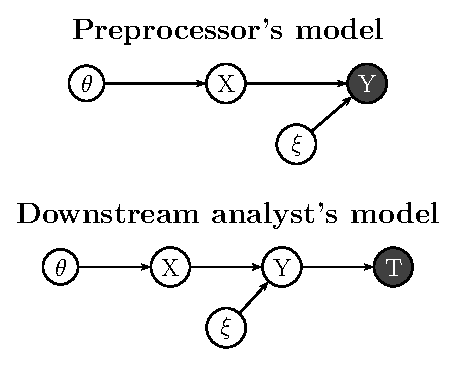
\includegraphics[height=2in]{figures/multiphase/diagram_model_vertical}
\caption{Graphical diagram of our  generic two-phase setting. The preprocessor  observes $Y$ from the original data generating process and outputs $T$, with $X$ as missing data. The downstream analyst observes the preprocessor's output $T$ and has both $X$ and $Y$ missing.\label{multiphase:fig:models}}
\end{figure}

This model incorporates   several restrictions.
First, it is Markovian with respect to $Y$, $X$, and $\param$; $Y$ is conditionally independent of $\param$ given $X$ (and $\obsparam$).
Second, the parameters governing the observation process ($\obsparam$) and those governing the scientific process  ($\param$) are distinct.
In Bayesian settings, we further assume that $\obsparam$ and $\param$ are independent \textit{a priori}.
The parameters $\obsparam$ are nuisance from the perspective of all involved; the downstream analyst wants to draw inferences about $X$ and $\param$, and the preprocessor wants to pass forward information that will be useful for said inferences.
If downstream inferences are Bayesian with respect to $\obsparam$, then $\pobs(Y|X) = \int \pobs(Y | X, \obsparam) \pi_\obsparam(\obsparam)\dd\mu_{\obsparam}(\obsparam)$ (which holds under (\ref{multiphase:e:model})) is sufficient for all inference under the given model and prior.
Hence, this conditional density is frequently of interest in our theoretical development, as is the corresponding marginalized model $p_{X,Y}(Y, X | \param) = \int \pobs(Y | X, \obsparam)  \psci(X | \param) \pi_\obsparam(\obsparam)\dd \mu_{\obsparam}(\obsparam)$.
We will compare results obtained with a fixed prior to those obtained in a more general setting to better understand the effects of nuisance parameters in multiphase inference.

These restrictions are somewhat similar to those underlying Rubin's \citeyearpar{Rubin1976} definition of ``missing at random''; however, we do not have missing data mechanism (MDM) in this setting \emph{per se}.
The distinction between missing and observed data ($X$ and $Y$) is fixed by the structure of our model.
In place of MDM, we have two imposed patterns of missingness: one for the data-generating process, and one for the inference process.
The first is $\pobs(Y \given X, \obsparam)$, which creates a noisy version of the desired scientific variables.
Here, $X$ can be considered the missing data and $Y$ the observed.
For the inference process, the downstream analyst observes $T$ in place of $Y$ but desires inference for $\param$ based upon $\psci(X | \param)$.
Hence, $Y$ and $X$ are both missing for the downstream analyst.
Neither pattern is entirely intrinsic to the problem---both are fixed by choice.
The selection of scientific variables $X$ for a given marginal likelihood $\pobs(Y | \param, \obsparam) = \int \pobs(Y | X, \obsparam) \psci(X | \param) \dd \mu_{X}(X)$ is a modeling decision.
The selection of preprocessing $T(Y)$ is a design decision.
This contrasts with the typical missing data setting, where MDM is forced upon the analyst by nature.
With multiphase problems, we seek to design and evaluate engineered missingness.
Thus the investigation of multiphase inference requires tools and ideas from design, inference, and computation in addition to the established theory of missing data.

\subsection{Defining multiphase procedures}
\label{multiphase:sec:def}

With this model in place, we turn to formally defining multiphase procedures.
This is more subtle than it initially appears.
In the MI setting, we focus on complete-data procedures for the downstream analyst's estimation and do not restrict the dependence structure between missing data and observations.
In contrast, we restrict the dependence structure as in (\ref{multiphase:e:model}), but place far fewer constraints on the analysts' procedures.
Here, we focus our definitions and discussion on the two phase case of a single preprocessor and downstream analyst.
This provides the formal structure to describe the interface between any two phases in a chain of multiphase analyses.

In our multiphase setting, downstream analysts need not have any complete-data procedure in the sense of one for inferring $\param$ from $X$ and $Y$; indeed, they need not formally have one based only upon $X$ for inferring $\param$.
We require only that they have a set of procedures for their desired inference using the quantities provided from earlier phases as inputs ($T$),  not necessarily  using direct observations of $X$ or $Y$.
Such situations are common in practice, as methods are often built around properties of preprocessed data such as smoothness or sparsity that need not hold for the actual values of $X$.

For the preprocessor, the input  is $Y$ and the output is $T$.
 Here  $T$ could consist of a vector of means with corresponding standard errors, or,  for discrete $Y$, $T$ could consist of carefully selected cross-tabulations.
In general, $T$ clearly needs to be related to $X$ to capture inferential information, but its actual form is influenced by practical constraints (e.g., aggregation to lower than desired resolutions due to data storage capacity).

For the downstream analyst, the input is $T$ and the output is an inference for $\theta$. 
This analyst can obviously adapt. 
For example, suppose $\param = E(X_i)$ for each entry $i$ of $X$.
If the preprocessor provides $T_0 = \hat{X}$, the analyst may simply use an unweighted mean to estimate $\param$.
If the preprocessor instead gives the analyst $T_1 = (\hat{X}, S)$, where $S$ contains standard errors, the latter could instead use a weighted mean to estimate $\param$.
This adaptation extends to an arbitrary number of possible inputs $T_k$, each of which corresponds to a set of constraints facing the preprocessor.

To formalize this notion of adaptation, we first define an index set $C$ with one entry for each such set of constraints.
This maps between forms of input provided by the preprocessor and estimators selected by the downstream analyst.
In this way, $C$ captures the downstream analyst's knowledge of previous processing and the underlying probability model.
Thus, this index set plays an central role in the definition of multiphase inference problems, far beyond that of a mere mathematical formality; it regulates the amount of mutual knowledge shared between the preprocessor and the downstream analyst.

Now, we turn to the estimators themselves.
We start with point estimation as a foundation for a broader class of problems.
Testing begins with estimating rejection regions, interval estimation with estimating coverage, classification with estimating class membership, and prediction with estimating future observations and, frequently, intermediate parameters.
The framework we present therefore provides tools that can be adapted for more than estimation theory.
We define multiphase estimation procedures as follows:
%
\begin{definition}
A \emph{multiphase estimation procedure} $\proc$ is a set of estimators $\{\est_k(T_k) : k \in C \}$ indexed by the set $C$, where $T_k$ corresponds to the output of the $k$th first-phase method; that is, $\proc$ is a family of estimators with different inputs.
\end{definition}
%
When clear, we will drop the subscripts $k$ and index the estimators in $\proc$ by their inputs.
This definition provides enough flexibility to capture many practical issues with multiphase inference, and it can be iterated to define procedures for analyses involving a longer sequence of preprocessors and analysts.
It also encompasses the  definition of a missing data procedure used by \citet{Meng1994}.
Such procedures cannot, of course, be arbitrarily constructed if they are to deliver results with general validity.
Hence, having defined these procedures, we will cull many of them from consideration in Section \ref{multiphase:sec:riskmonotone}.

The obvious choice of our estimand, suggested by our notation thus far, is the parameter for the scientific model, $\param$.
This is very amenable to mathematical analysis and relevant to many investigations.
Hence, it forms the basis for our results in Section \ref{multiphase:sec:theory}.
However, for multiphase analyses, other classes of estimands may prove more useful in practice.
In particular, functions of $X$, future scientific variables $X_{rep}$, or future observations $Y_{rep}$ may be of interest.
Prediction of such quantities is a natural focus in the multiphase setting because such statements are meaningful to both the preprocessor and downstream analyst.
% Statements about future observations $Y_{rep}$ and latent quantities $X$ then have the same meaning to both analysts.
Such estimands naturally encompass a broad range of statistical problems including prediction, classification, and clustering.
However, there is often a lack of mutual knowledge about $\psci(X \given \param)$, so the preprocessor cannot expect to ``target'' estimation of $\param$ in general, as we shall discuss in Section \ref{multiphase:sec:remarks}.


\subsection{When is more better?}
\label{multiphase:sec:riskmonotone}

It is not automatic for multiphase estimation procedures to produce better results as the first phase provides more information.
To obtain a sensible context for theoretical development, we must regulate the way that the downstream analyst adapts to different inputs.
For instance, they should obtain better results (in some sense) when provided with higher-resolution information.
This carries over from the MI  setting \citep{Meng1994,Meng2003,Meng2012,Xie2012}, where notions such as self-efficiency are useful for regulating the downstream analyst's procedures.
We define a similar property for multiphase estimation procedures, but without restricting  ourselves to the missing data setting. 
Specifically, let $T_1 \preceq T_2$ indicate $T_1$ is a deterministic function of $T_2$.
In practice, $T_1$ could be a subvector, aggregation, or other summary of $T_2$.
%
\begin{definition}[Risk monotonicity]
A multiphase estimation procedure $\proc$ is \emph{risk monotone} with respect to a loss function $L$ if, for all pairs of outputs $T_1, T_2$, $T_1 \preceq T_2$ implies $R(\est_2(T_2), L) \leq R(\est_1(T_1), L)$.
\end{definition}
%
An asymptotic analogue of risk monotonicity is defined as would be expected, scaling the relevant risks at an appropriate rate to obtain nontrivial limits.
This is a natural starting point for regulating multiphase estimation procedures; stronger notions may be required for certain theoretical results.
Note that this definition does not require that ``higher-quality'' inputs necessarily lead to lower risk estimators.
Risk monotonicity requires only that estimators based upon a larger set of inputs perform no worse than those with strictly less information (in a deterministic sense).
However, risk monotonicity is actually quite tight in another sense.
It requires that additional information cannot be misused by the downstream analyst, imposing a strong constraint on mutual knowledge.
For an example, consider the case of unweighted and weighted means.
To obtain better results when presented with standard errors, the downstream analyst must know that they are being given (the correct) standard errors and to weight by inverse variances.

This definition is related to the comparison of experiments, as explored by \citet{Blackwell51,Blackwell53}, but diverges on a fundamental level.
Our ordering of experiments, based on deterministic functions, is more stringent than that of \cite{Blackwell53}, but they are related.
Indeed, our $\preceq$ relation implies that of \citet{Blackwell53}.
In the latter work, an experiment $\alpha$ is defined as more informative than experiment $\beta$, denoted $\alpha \supset \beta$, if all losses attainable from $\beta$ are also attainable from $\alpha$.
This relation is also implied if $\alpha$ is sufficient for $\beta$.
Our stringency stems from our broader objectives in the multiphase setting.
From a decision-theoretic perspective, the partial ordering of experiments investigated by Blackwell and others deal with which risks are attainable given pairs of experiments, allowing for arbitrary decision procedures.
In contrast, our criterion restricts procedures based on whether such risks are actually attained, with respect to a particular loss function.
This is because, in the multiphase setting, it is not generally realistic to expect downstream analysts to be capable of obtaining optimal estimators for all forms of preprocessing.

The conceptually-simplest way to generate such a procedure is to begin with a complete probability model for $\pobs(Y | \param)$.
Under traditional asymptotic regimes, all procedures consisting of Bayes estimators based upon such a model will (with full knowledge of the transformations involved in each $T_k$ and a fixed prior) be risk monotone.
The same is true asymptotically under the same regimes (for squared-error loss) for procedures consisting of MLEs under a fixed model.
Under some other asymptotic regimes, however, these principles of estimation do not guarantee risk-monotonicity; we explore this further in Section \ref{multiphase:sec:missinfo}.
But such techniques are not the only way to generate risk monotone procedures from probability models.
This is analogous to self-efficiency, which can be achieved by procedures that are neither Bayesian nor MLE \citep{Meng1994,Xie2012}.

\begin{figure}
\centering
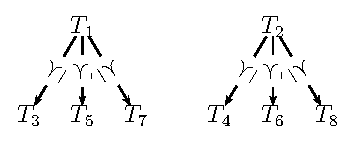
\includegraphics[height=1in]{figures/multiphase/diagram_risk-monotone.eps}
\caption{Illustration of risk-monotone ``basis'' construction. In this case, $T_1$ and $T_2$ form the basis set of statistics. Each of these has three descendants ($T_3, T_5, T_7$ from $T_1$ and $T_4, T_6, T_8$ from $T_2$). These descendants are deterministic functions of their parent, but they are not deterministic functions of any other basis statistics. Given correctly-specified models for $T_1$ and $T_2$, a risk monotone procedure can be constructed for all statistics ($T_1, \ldots, T_8$) shown here as described in the text.
\label{multiphase:fig:risk-monotone}}
\end{figure}

A risk monotone procedure can be generated from any set of probability models for distinct inputs that ``span'' the space of possible inputs.
Suppose that an analyst has a set of probability models, all correctly specified, for $p_{T_b}(T_b | \param)$, where $b$ ranges over a subset $B$ of the relevant index set $C$.
We also assume that this analyst has a prior distribution $\pi_b(\param)$ for each such basis models.
These priors need not agree between models; the analyst can build a risk-monotone procedure from an inconsistent set of prior beliefs.
Suppose that the inputs $\{T_b : b \in B\}$ are not deterministic functions of each other and all other inputs can be generated as nontrivial deterministic transformations of one of these inputs.
Formally, we require $T_b \not \preceq T_c$ for all distinct $b, c \in B$ and, for each $k \in C$ there exists a unique $b \in B$ such that $T_k \preceq T_b$ (each output is uniquely descended from a single $T_b$),
as illustrated  in Figure \ref{multiphase:fig:risk-monotone}.
This set can form a basis, in a sense, for the given procedure.

Using the given probability models with a single loss function and set of priors (potentially different for each model), the analyst can derive a Bayes rule under each model.
For each $b \in B$, we require $\est(T_b)$ to be an appropriate Bayes rule on said model.
As $T_k = g_k(T_b)$ for some function $g_k$, we then have the implied $p_{T_k}(T_k | \param) = \int_{t : g_k(t) = T_k} p_{T_b}(t | \param) \dd t$, yielding the Bayes rule for estimating $\param$  based on $T_k$, which is no less risky than $\est(T_b)$.
The requirement that each output $T_k$ derives from a unique $T_b$ means that each basis component $T_b$ has a unique line of descendants.
Within each line, each descendant is comparable to only a single $T_b$ in the sense of deterministic dependence.
Between these lines, such comparisons are not possible.
This ensures  the overall risk-monotonicity.

Biology provides an illustration of such bases.
A wide array of methodological approaches have been used to analyze high-throughput gene expression data.
One approach, builds upon order and rank statistics \citep{Geman2004,Tan2005,Geman2012}.
Another common approach uses differences in gene expression between conditions or experiments, often aggregating over pathways, replicates, and so forth.
Each class of methods is based upon a different form of preprocessing: ranks transformations for the former, normalization and aggregation for the latter.
Taking procedures based on rank statistics and aggregate differences in expression as a basis, we can consider constructing a risk-monotone procedure as above.
Thus, the given formulation can bring together apparently disparate methods as a first step in analyzing their multiphase properties.

Such constructions are, unfortunately, not sufficient to generate all possible risk monotone procedures.
Obtaining more general conditions and constructions for risk monotone procedures is a topic for further work.

\subsection{Revisiting our examples and probing our boundaries}
\label{multiphase:sec:revisit}

By casting the examples in Section \ref{multiphase:sec:examples} into the formal structure just established, we can clarify the practical role of each mathematical component and see how to map theoretical results into applied guidance.
We also provide an example  that illustrates the boundaries of the framework's utility, and another that demonstrates its formal limits.
These provide perspective on the trade-offs made in formalizing the multiphase inference problem. 

The case of microarray preprocessing presented previously fits quite nicely into the model of Section \ref{multiphase:sec:model}.
There, $Y$ corresponds to the observed probe-level intensities, $X$ corresponds to the true expression level for each gene under each condition, and $\param$ corresponds to the parameters governing the organism's patterns of gene expression.
In the microarray setting, $\pobs$ would characterize the relationship between expression levels and observed intensities, governed by $\obsparam$.
These nuisance parameters could include chip-level offsets, properties of any additive background, and the magnitudes of other sources of variation.
The assumptions of a Markovian dependence structure and distinct parameters for each part of the model appear quite reasonable in this case, as (1) the observation $Y$ can only (physically) depend upon the sample preparation, experimental protocol, and RNA concentrations in the sample and (2) the distributions $\psci$ and $\pobs$ capture physically distinct portions of the experiment.
Background correction, normalization, and the reduction of observations to log-fold changes are common examples of preprocessing $T(Y)$. As discussed previously, estimands based upon $X$ may be of greater scientific interest than those based upon $\param$.
For instance, we may want to know  whether gene expression changed between two treatments in a particular experiment (a statement about $X$) than whether a parameter regulating the overall patterns of gene expression takes on a particular value.

For the astrophysical example, the fit is similarly tidy.
The raw astronomical observations correspond to $Y$, the true temperature, density, and spectral properties of each part of the dust cloud become $X$, and the parameters governing the relationship between these quantities (e.g., their correlation) form $\param$.
The $\pobs$ distribution governs the physical observation process, controlled by $\obsparam$.
This process typically includes the instruments' response to astronomical signals, atmospheric distortions, and other earthbound phenomena.
As before, the conditional independence of $\param$ and $Y$ given $X$ and $\obsparam$ is sensible based upon the problem structure, as is the separation of $\param$ and $\obsparam$. Here  $X$ corresponds to signals emitted billions or trillions of miles from Earth, whereas the observation process occurs within ground- or space-based telescopes.
Hence, any non-Markovian effects are quite implausible.
Preprocessing $T(Y)$ corresponds to the (point) estimates of temperature, density, and spectral properties from simple models of $Y$ given $X$ and $\obsparam$.

The multiphase framework encompasses a broad range of settings, but it does not shed additional light on all of them.
If $T$ is a many-to-one transformation of $Y$, then our framework implies that the preprocessor and downstream analyst face structurally  different inference (and missing data) problems.
This is the essence of multiphase inference, in our view.
Settings where $\pobs(Y|X, \obsparam)$ is degenerate or $T$ is a one-to-one function of $Y$ are boundary cases where our multiphase interpretation and framework add little.

For a concrete example of these cases, consider a time-to-failure experiment, with the times of failure $W_i \sim \,\mbox{i.i.d}\, \Expo(\param)$, $i = 1, \ldots, n$.
Now, suppose that the experimenters actually ran the experiment in $m$ equally-sized batches.
They observe each batch only until its first failure; that is, they observe and report $Y_b = \min \{W_i : i \mbox{ in batch } b \}$ for each batch $b$.
Subsequent analysts have access only to $T = (Y_1, \ldots, Y_b)$.
This seems to be a case of preprocessing, but it actually resides at the very edge of our framework.

We could take the complete observations to be $X$ and the batch minima to be $Y$.
This would satisfy our Markov constraint, with a singular, and hence deterministic, observation process $\pobs(Y | X)$ simply selecting a particular order statistic within each batch.
However, $T(Y)$ is one-to-one; the preprocessor observes only the order statistics, as does the downstream analyst.
There is no separation of inference between phases; the same quantities are observed and missing to both the preprocessor and the downstream analyst.
Squeezing this case into the multiphase framework is technically valid but unproductive.

The framework we present is not, however, completely generic.
Consider a chemical experiment involving a set of reactions.
The underlying parameters $\param$ describe the chemical properties driving the reactions, $X$ are the actual states of the reaction, and $Y$ are the (indirectly) measured outputs of the reactions.
The measurement process for these experiments, as described by $\pobs(Y|X, \obsparam)$, could easily violate the structure of our model in this case.
For instance, the same chemical parameters could affect both the measurement and reaction processes, violating the assumed separation of $\param$ and $\obsparam$.

Even careful preprocessing in such a setting can create a fundamental incoherence.
Suppose the downstream analysis will be Bayesian, so the preprocessor provides the conditional density of $Y$ as a function of $X$, $\pobs(Y | X)$,  for the observed $Y$.
If $\param$ and $\obsparam$ share components, and the preprocessor uses their prior on $\obsparam$ to create $\pobs(Y | X)$, the conditional density need not be sufficient for $\param$ under the downstream analyst's model.
Because the downstream analyst's prior on $\param$ need not be compatible with the preprocessor's prior on $\obsparam$, inferences based on the preprocessor's $\pobs(Y | X)$ can be seriously flawed in this setting.
Hence, we exclude such cases from our investigation for the time being.

Thinking Bayesianly, our model  (\ref{multiphase:e:model}) obviously  does not exclude the possibility that the downstream analyst has more knowledge about $\param$ than the preprocessor in the form of a prior on $\theta$.
However, \textit{prior} information means that it is based on studies that do not overlap with the current one.
Probabilistically  speaking,  this means that our model permits the downstream analyst to formally incorporate  another data set $Z$,  as long as $Z$ is conditionally independent of the scientific variables $X$ and observations $Y$ given $(\param, \obsparam)$ or $\param$.
For example, the downstream analyst could observe completely separate experiments pertaining to the same underlying process governed by $\param$ or the outcomes of separate calibration pertaining to $\obsparam$, but not additional replicates governed by the same realization of $X$.
In a biological setting, this means that the downstream analyst could have access to results from samples not available to the preprocessor (e.g., biological replicates), possibly using the same equipment; however, they could not have access to additional analyses of the same biological sample (e.g., technical replicates), as a single biological sample would typically correspond to a single realization of $X$.

These examples remind us that our multiphase setting does not encompass all of statistical inference.
This is quite a relief to us.
Our work aims to open new directions for statistical research, but it cannot possibly address every problem under the sun!

\subsection{Constraints will set your theory free}
\label{multiphase:sec:constraints}

Multiphase theory hinges on procedural constraints.
Consider, for example, finding the optimal multiphase estimation procedure in terms of the final estimator's Bayes risk.
Without stringent procedural constraints, the result is trivial: compute the appropriate Bayes estimator using the distribution of $T$ given $\param$.
Similarly, the optimal preprocessing $T$ will, without tight constraints, simply compute an optimal estimator using $Y$ and pass it forward.
Note that both of these cases respect risk-monotonicity to the letter; it is not sufficiently tight to enable interesting, relevant theory.
% This pattern repeats across many inquiries, with both Bayesian, frequentist, and asymptotic techniques and for both phases.
More constraints, based upon careful consideration of applied problems, are clearly required.

This is not altogether bad news.
We need only look to the history of multiple imputation to see how rich theory can arise from stringent, pragmatic constraints.
Multiple imputation forms a narrow subset of multiphase procedures: $X$ corresponds to the complete data ($Y_{com}$, in MI notation), $Y$ corresponds to the observed data $Y_{obs}$ and missing data indicator $R$, and $T$ usually consists of posterior predictive draws of the missing data together with the observed data.
The Markovian property depicted in Figure~\ref{multiphase:fig:models} holds when the parameter ($\xi$) for the missing data mechanism $p(R|Y_{com},\xi$) is distinct from the parameter of interest ($\theta$) in $p(Y_{com}|\theta)$, which is a common assumption in practice.
The second-phase procedure is then restricted to repeatedly applying a complete-data procedure and combining the results.
These constraints were originally imposed for practical reasons---in particular, to make the resulting procedure feasible with existing software.
However, they have opened the door to deep theoretical investigations.

In that spirit, we consider two types of practically-motivated constraints for multiphase inference: restrictions on the downstream analyst's procedure and restrictions on the preprocessor's methods.
These constraints are intended to work in concert with coherence conditions (e.g., risk monotonicity), not in isolation, to enable meaningful theory.

Constraints on the downstream analyst are intended to reflect practical limitations of their analytic capacity.
Examples  include restricting the downstream analyst to narrow classes of estimators (e.g., linear functions of preprocessed inputs), to specific principles of estimation (e.g., MLEs), or to special cases of a method we can reasonably assume the downstream analyst could handle, such as a complete-data estimator $\est(X)$, available from software with appropriate inputs.
Estimators derived from nested families of models are often suitable for this purpose.
For example, whereas $\est(X)$ may involve only an ordinary regression, the computation of  $\est(T)$ may require  a weighted least-squares regression.
%This is an example of  constructing  a reasonably constrained procedure, specializing a feasible estimator to generate a wide family of options.
% All of these constraints can rule out many forms of adaptation, enabling richer theory.

Another constraint on the downstream analyst pertains to nuisance parameters.
Such constraints are of great practical and theoretical interest, as we believe that the preprocessor will typically have better knowledge and statistical resources available to address nuisance parameters than the downstream analyst.
An extreme but realistic case of this is to assume that the downstream analyst cannot address nuisance parameters at all.
As we shall discuss in Section \ref{multiphase:sec:theory}, this would force the preprocessor to either marginalize over the nuisance parameters, find a pivot with respect to them, or trust the downstream analyst to use a method robust to the problematic parameters.

Turning to the preprocessor, we consider restricting either the form of the preprocessor's output or the mechanics of their methods.
In the simplest case of the former, we could require that $T$ consist of the posterior mean ($\hat{X}$) and posterior covariance ($V$) of the unknown $X$ under the preprocessor's model.
A richer, but still realistic, class of output would be finite-dimensional real or integer vectors.
Restricting output to such a class would prevent the preprocessor from passing arbitrary functions onto the downstream analyst.
This leads naturally to the investigation of (finite-dimensional) approximations to the preprocessor's conditional density, aggregation, and other such techniques.

On the mechanical side, we can restrict either the particulars of the preprocessor's methods or their broader properties.
Examples of the former include particular computational approximations to the likelihood function or restrictions to particular principles of inference (e.g., summaries of the likelihood or posterior distribution of $X$ given $(Y, \obsparam)$).
Such can focus our inquiries to specific, feasible methods of interest or reflect the core statistical principles we believe the preprocessor should take into account.
In a different vein, we can require that preprocessor's procedures be distributable across multiple researchers, each with their own experiments and scientific variables of interest.
Such settings are of interest for both the accumulation of scientific results for later use and for the development of distributed statistical computation.
This leads to preprocessing based upon factored ``working'' models for $X$, as we explore further in Section \ref{multiphase:sec:sufficiency}.
Nuisance parameters play an important role in these constraints, narrowing the class of feasible methods (e.g., marginalization over such parameters may be exceedingly difficult) and largely determining the extent to which preprocessing can be distributed.
We explore these issues in more detail throughout Section \ref{multiphase:sec:theory}.

\section{A few theoretical cornerstones}
\label{multiphase:sec:theory}

We now present a few steps towards a theory of multiphase inference.
In this, we endeavor to address three basic questions: (1) how can we determine what to retain, (2) what limits the performance of multiphase procedures, and (3) what are some minimal requirements for being an ideal preprocessor?
We find insight into the first question from the language of classical sufficiency.
We leverage and specialize results from the missing-data literature  to address the second.
For the third question, we turn to the tools of decision theory.

\subsection{Determining what to retain}
\label{multiphase:sec:sufficiency}

Suppose we have a group of researchers, each with their own experiments.
They want to preprocess their data to reduce storage requirements, ease subsequent analyses, and (potentially) provide robustness to measurement errors.
This group is keenly aware of the perils of preprocessing and want to ensure that the output they provide will be maximally useful for later analyses.
Their question is, ``Which statistics should we retain?''

If each of these researchers was conducting the final analysis themselves, using only their own data, they would be in a single-phase setting.
The optimal strategy then is  to keep a minimal sufficient statistic for each researcher's model. 
Similarly, if the final analysis were planned and agreed upon among all researchers, we would again have a single-phase setting,  and  it is optimal to retain the sufficient statistics for the agreed-upon model.
We use the term \textit{optimal} here because it achieves maximal data reduction without losing information about the parameters of interest.
Such lossless compression--in the general sense of avoiding statistical redundancy--is often impractical, but it provides a useful theoretical gold standard.%upper bound on what we can possibly aim for.

In the multiphase setting, especially with multiple researchers in the first phases, achieving optimal preprocessing is far more complicated even in theory.
If $T(Y)$ is  the output of the \textit{entire} preprocessing phase, then in order to retain all information we must require $T(Y)$ to be a sufficient statistics for $\{\theta,\xi\}$ under model (\ref{multiphase:e:model}); that is, 
\begin{equation}\label{multiphase:e:con1}  
L(\theta,\xi|T(Y))=L(\theta,\xi|Y),
\end{equation}
where $L$ denotes a likelihood function;  or at least in the (marginal) Bayesian sense,
\begin{equation}\label{multiphase:e:con2}
P(\theta|T(Y))=P(\theta|Y),
\end{equation}
where $P(\theta|D)$ is the posterior of $\theta$ given data $D$ with the likelihood given by  (\ref{multiphase:e:model}).
Note  that (\ref{multiphase:e:con1}) implies (\ref{multiphase:e:con2}), and (\ref{multiphase:e:con2}) is useful when the downstream analyst wants only a Bayesian inference of $\theta$.
In either case the construction of the sufficient statistic generally depends on the joint model for $Y$ as implied by (\ref{multiphase:e:model}), requiring more knowledge than individual researchers typically possess.

Often, however, it is reasonable to assume the following conditional independence.
Let $\{Y_i, X_i, \obsparam_i\}$ be the specification of $\{Y, X, \obsparam\}$ for researcher $i\ (=1,\ldots, r)$, where $\{Y_1,\ldots, Y_r\}$ forms a \textit{partition} of $Y$.  We then assume that
\begin{equation}\label{multiphase:e:obsm}
 \pobs(Y | X, \obsparam)= \prod_{i=1}^r p_{Y_i}(Y_i | X_i, \obsparam_i)\ .
\end{equation}
Note in the above definition implicitly we also assume the baseline measure $\mu_Y$ is a product measure $\prod_{i=1}^r \mu_{Y_i}$, such as Lebesgue measure.
The assumption (\ref{multiphase:e:obsm}) holds, for example, in microarray applications, when different labs provide conditionally-independent observations of probe-level intensities.
The preceding discussion suggests that this assumption is necessary for ensuring (\ref{multiphase:e:con1}) or even (\ref{multiphase:e:con2}), but obviously it is far from sufficient because it says nothing about the model on $X$.

It is reasonable---or at least more logical than not---to assume each researcher has the best knowledge to specify  his/her own observation model $p_{Y_i}(Y_i | X_i, \obsparam_i)$ ($i=1,\ldots, r)$.
But, for the scientific model $p_X(X|\theta)$ used by the downstream analyst, the best we can hope is that each researcher has \textit{a working model} $\tilde p_X(X_{i}|g_i(\eta))$ that is in some way related to $p_X(X|\theta)$.
The notation $g_i(\eta)$ reflects our hope to construct a common working parameter $\eta$ that can ultimately be \textit{linked} to the scientific parameter $\theta$.
 
Given this working model, the $i$th researcher can obtain the corresponding (minimal) sufficient statistic $T_i(Y)$ for $\{ g_i(\workparam), \xi_i\}$ with respect to 
\begin{equation}\label{multiphase:e:prob}
  \pwork(Y_i | g_i(\workparam), \obsparam_i) = \int \pobs(Y_i | X_i, \obsparam_i) \pwork(X_i | g_i(\workparam)) \dd \mu_{X_i}(X_i), \quad i=1,\ldots, r.
\end{equation}
When one has a prior $ \pi_{\obsparam_i}(\obsparam_i)$ for  $\xi_i$, one could alternately decide to retain the (Bayesian) sufficient statistic $T_i^{B}(Y_{i})$ with respect to the model 
\begin{equation}\label{multiphase:e:prom}
  \pywork(Y_i | g_i(\workparam)) = \int \int \pobs(Y_i | X_i, \obsparam_i) \pwork(X_i | g_i(\workparam)) \pi_{\obsparam_i}(\obsparam_i) \dd \mu_{X_i}(X_i) \dd \mu_\obsparam(\obsparam_i)\ .
\end{equation} 

Our central interest here is to determine when the collection $T(Y)=\{T_i(Y_i): i=1,\ldots, r\}$ will satisfy (\ref{multiphase:e:con1}) and when $T^{B}(Y)=\{T_i^B(Y_i): i=1,\ldots, r\}$ will satisfy (\ref{multiphase:e:con2}).
This turns out to be an exceedingly difficult problem if we seek a necessary and sufficient condition for \textit{when} this occurs.
However, it is not difficult to identify sufficient conditions that can provide useful practical guidelines.
We proceed by first considering cases where $\{X_1, \ldots, X_r\}$ forms a partition of $X$.
Compared to the assumption on partitioning $Y$, this assumption is less likely to hold in practice because different researchers can share common  parts of $X$'s or even  the entire  scientific variable $X$.
% Fortunately, it turns out that the results we obtain also shed light on more general cases, as we shall demonstrate later.
However, as we shall demonstrate shortly,  we can extend our results formally to all models for $X$, as long as we are willing  to put tight restrictions on the allowed class of working models.
Specifically, the following condition describes a class of working models that are ideal because they permit separate preprocessing yet retain joint information.
 Note again that an implicit assumption here is that the baseline measure $\mu_X$ is a product measure $\prod_{i=1}^r\mu_{X_i}$.
\begin{definition}
[Distributed Separability Condition (DSC)]
A set of working models $\{\pwork(X_i |g_{i}(\workparam)): i=1,\ldots, r\}$ is said to satisfy the \emph{distributed separability condition} with respect to $\psci(X | \param)$ if there exists a probability measure $p_\workparam( \workparam | \param)$ such that
\begin{equation}
 \psci(X | \param)\ = \int_\eta\left[ \prod_{i=1}^r \pwork(X_i | g_i(\workparam)) \right]\dd p_\workparam(\workparam | \param).\  \label{multiphase:eq:dsc}
\end{equation}
\end{definition}

% We also assume that each researcher can correctly specify a scientific model for their data---that is, they know $\psci(X_i | \param)$.


\begin{theorem}
\label{multiphase:thm:dsc}
Under the assumptions (\ref{multiphase:e:obsm}) and (\ref{multiphase:eq:dsc}), we have 
\begin{itemize}
\item[(1)] The collection of individual sufficient statistics from (\ref{multiphase:e:prob}), that is, $T(Y)=\{T_i(Y_i), i=1,\ldots, r\}$,  is  jointly sufficient for $\{\theta,\xi\}$ in the sense  that  (\ref{multiphase:e:con1}) holds.
\item[(2)] Under the additional assumption that $\{\xi_1,\ldots, \xi_r\}$ forms a partition of $\xi$ and $\pi(\xi)\dd \mu_{\xi}=\prod_{i=1}^r \pi_{\xi_i}(\xi_i)\dd\mu_{\xi_i}$, both $T(Y)$ corresponding to (\ref{multiphase:e:prob}) and $T^B(Y)$ corresponding to  (\ref{multiphase:e:prom}) are Bayesianly sufficient  for $\theta$  in the sense that (\ref{multiphase:e:con2}) holds. 
\end{itemize}
\end{theorem}
% TODO:+DONE AWB, Brief proof -> appendix.
%       Connection with exchangability. Stronger and weaker, in some ways.
%       \eta -> (\eta_1, ..., \eta_r) as one-to-many map
%       Same for X -> (X_1, ..., X_r)
%       Common spaces; replaces partitions
%       
\begin{proof}
 By the sufficiency of $T_i$ for $(g_i(\workparam), \obsparam_i)$, we can write
\begin{equation}\label{multiphase:eq:a1}
  \int_{X_i} \pobs(Y_i | X_i, \obsparam_i) \pwork(X_i | g_i(\workparam)) \dd\mu_{X_i}(X_i) = \pywork (Y_i | g_i(\workparam), \obsparam_i) =h_i(Y_i) f_i(T_i ; g_i(\workparam), \obsparam_i).
\end{equation}
This implies that, 
\begin{align*}
\pobs(Y | \param, \obsparam) =&  \int_{X} \pobs(Y | X, \obsparam) \psci(X | \param)\dd \mu_X(X) \\
[{\rm by}\ (\ref{multiphase:e:obsm}) \ {\rm and}\ (\ref{multiphase:eq:dsc})]\ =& \int_{X} \left[ \prod_{i=1}^{r} \pobs(Y_i | X_i, \obsparam_i) \right] \cdot \\
& \left[ \int_{\eta} \left[ \prod_{i=1}^{r} \pwork(X_i | g_i(\workparam)) \right]\dd p_\workparam(\workparam | \param) \right]\dd \mu_X(X) \\
[{\rm by\ factorization\ of} \ \mu_X]\ =& \int_{\eta} \prod_{i=1}^{r} \left[ \int_{X_i} \pobs(Y_i | X_i, \obsparam_i) \pwork(X_i | g_i(\workparam))\dd \mu_{X_i}(X_i) \right]\dd p_\workparam(\workparam | \param)  \\ 
[{\rm by}\ (\ref{multiphase:eq:a1})] =& \left[ \prod_{i=1}^{r} h_i(Y_i) \right] \left[ \int_{\eta} \prod_{i=1}^{r} f_i(T_i;g_i(\workparam), \obsparam_i)\dd p_\workparam(\workparam | \param)\right] .
\end{align*}
This establishes (1) by the factorization theorem. 
Assertion (2) is easily established via an analogous argument, by integrating all the expressions above with respect to $\pi(\xi)\dd\mu(\xi)=\prod_{i=1}^r \pi_{\xi_i}(\xi_i)\dd \mu_{\xi_i}(\xi_i)$. 
\end{proof}

%
We emphasize that DSC does not require individual researchers to model their parts of $X$ in the same way as the downstream analyst would, which would make it an essentially tautological condition.
Rather, it requires that individual  researchers understand their own problems and how they can fit into the broader analysis hierarchically.
This means that the working model for each $X_i$ $(i=1,\ldots, r)$ can be more saturated than the downstream analyst's model for the same part of $X$.

Consider a simple case with $r=1$, where  the preprocessor correctly assumes the  multivariate normality for $X$ but is unaware that its covariance actually has a block structure or is unwilling  to impose such a restriction to allow for more flexible downstream analyses. 
Clearly any sufficient statistic under the unstructured multivariate model is also sufficient for any (nested) structured ones.
The price paid here is failing to achieve the greatest possible sufficient reduction of the data, but this sacrifice may be necessary to ensure the broader validity of downstream analyses.
For example, even if  downstream analysts adopt a block-structured covariance, they  may still want to perform a model checking, which would not be possible if all they are given is a \textit{minimal}  sufficient statistic for the model to be checked.    


Knowledge suitable for specifying a saturated model is more attainable than complete knowledge of $\psci(X | \param)$, although ensuring common knowledge of its (potential) hierarchical structure  still requires some coordination among the researchers.
Each of them could independently determine for which classes of scientific models their working model satisfies the DSC.
However, without knowledge of the partition of $X$ across researchers and the overarching model(s) of interest, their evaluations need not provide  any useful consensus.
This suggests the necessity of some general communications and a practical guideline for distributed preprocessing, even when we have chosen a wise  division of labors that permits DSC to hold.

Formally, DSC is similar in flavor to de Finetti's theorem, but it does not require the components of the factorized working model to be exchangeable. 
DSC, however, is by no means necessary (even under (\ref{multiphase:e:con1})), as an example in Section \ref{multiphase:sec:counterexamples} will demonstrate.
Its limits stem from ``unparameterized'' dependence---dependence between $X_i$'s that is not controlled by $\param$.
When such dependence is present, statistics can exist that are sufficient for both $\workparam$ and $\param$ without the working model satisfying DSC.

However, a simple necessary condition for distributed sufficiency is available.
 Unsurprisingly, it links the joint sufficiency of $T(Y)=\{T_i(Y_i): i=1,\ldots, r\}$ under $p_{Y}(Y|\theta)$ to the joint sufficiency of $S(X)=\{S_i(X_i), i=1,\ldots,r\}$ under the scientific model $p_X(X|\theta)$, where $S_i(X_i)$ is any sufficient statistic for the working model $\tilde p_X(X_{i}|g_i(\eta)), i=1,\ldots, r$.
%
\begin{theorem}
\label{multiphase:thm:necessary}
If, for all observation models satisfying (\ref{multiphase:e:obsm}), the collections of individual sufficient statistics from (\ref{multiphase:e:prob}) $T(Y)=\{T_i(Y_i), i=1,\ldots, r\}$ are jointly sufficient for $\{\theta,\xi\}$ in the sense that  (\ref{multiphase:e:con1}) holds, then any collection of individual sufficient statistics under $\{\pwork(X_i | g_i(\eta)), i=1,\ldots, r\}$, that is, $S(X)$, must be sufficient for $\theta$ under $\psci(X | \theta)$.
\end{theorem}
%
The proof of this condition emerges easily by considering the trivial observation model $\pobs(Y_i | X_i, \xi) = \delta_{\{Y_i = X_i\}}$, where $\delta_{A}$ is the indicator function of set $A$.
Theorem \ref{multiphase:thm:necessary} holds even if we require the observation model to be nontrivial, as the case of $\pobs(Y_i | X_i, \xi) \propto \delta_{\{Y_i \in B_{\varepsilon}[X_i]\}}$ for arbitrary $\varepsilon$-neighborhoods of $X_i$ demonstrates.
The result says that if we want distributed preprocessing to provide a lossless compression regardless of the actual form of the observation model, then even under the conditional independence assumption (\ref{multiphase:e:obsm}), we must require the individual working models to  \textit{collectively} preserve sufficiency under the scientific model.
 Note that preserving sufficiency for a model is a much weaker requirement than preserving the model itself.
Indeed, two models can have very different model spaces yet share the same \textit{form} of sufficient statistics, as seen with i.i.d.
$\Poisson(\mu)$ and $N(\mu, 1)$ models, both yielding the sample average as a complete sufficient statistic.

Although we find this sufficiency-preserving condition quite informative about the limits of lossless distributed preprocessing, it is not a sufficient condition.
As a counterexample, consider  $Y_{ij} | X_i \sim N(\mu_i, \sigma_{ij}^2 )$ independent for $i=1,\ldots,n$, $j=1,\ldots,m$, where $X_i \equiv (\mu_i, \sigma_{i1}^2, \ldots, \sigma_{im}^2)$.
For the true model, we assume $\psci(X|\theta)$ as
follows: $\mu_i | \theta \sim N(\theta, 1)$, $\sigma_{ij}^2 \sim 1/{\chi_1}^2$, and all variables are mutually  independent.
For the working model, we take $\pwork(X|\eta)$ as
follows: $\mu_i | \eta_i \sim N(\eta_i, 1)$ independently, and $\sigma_{ij}^2 = 1$ with probability 1 for all $i,j$.
%
Obviously $S=(\mu_1, \ldots, \mu_n)$ is a sufficient statistic for both $\pwork(X|\eta)$ and $p_X(X|\theta)$ because of their normality. Because $S$ is \textit{minimally} sufficient for $\eta$, this implies that any sufficient statistic for $\pwork(X|\eta)$ must be sufficient for $p_X(X|\theta)$, therefore the sufficiency preserving condition holds.

However,  the collection of the complete sufficient statistics $T_i =  \, \sum_j y_{ij}/m, i=1, \ldots, r$ for  $\eta$ under $p_Y(Y|\eta)$ is not sufficient for $\theta$ under $\pobs(Y | \theta)$ because the latter is no longer an exponential family.
The trouble is caused by the failure of the working models to capture additional flexibility in the scientific model that is not controlled by  its parameter $\theta$.
 Therefore, obtaining a condition that is both necessary and sufficient for lossless compression via distributed preprocessing is a challenging task.
Such a condition appears substantially more intricate than those presented in Theorems \ref{multiphase:thm:dsc} and \ref{multiphase:thm:necessary} and may therefore be less useful as an applied guideline.
%Theoretical intricacies like these seem to be rules rather than exceptions with multiphase inferences.
Below we discuss a few further subtleties.
  
\medskip
\noindent
{\bf Likelihood sufficiency verses Bayesian efficiency.}
Although Theorem~\ref{multiphase:thm:dsc} covers both likelihood and Bayesian cases, it is important to note a subtle distinction between their general implications.
 In the likelihood setting (\ref{multiphase:e:con1}), we achieve lossless compression for all downstream analyses targeting $(\param, \obsparam)$.
 This allows the downstream analyst to obtain inferences that are robust to the preprocessor's beliefs about $\obsparam$, and they are free to revise their inferences if new information about $\obsparam$ becomes available.
But, the downstream analyst must address the nuisance parameter $\xi$ from the preprocessing step, a task a downstream analyst may not be able or willing to handle.

In contrast, the downstream analyst need not worry about $\xi$ in the Bayesian setting (\ref{multiphase:e:con2}).
However, this is archived at the cost of robustness.
All downstream analyses are potentially affected by the preprocessors' beliefs about $\xi$.
Furthermore, because $T^B(Y)$ is required only to be sufficient for $\theta$,  it may not carry any information for a downstream analyst to check the preprocessor's assumptions about $\obsparam$.
Fortunately, as it is generally logical to expect the preprocessor to have better knowledge addressing $\xi$ than the downstream analyst, such robustness may not be a serious concern from a practical perspective.
Theoretically, the trade-off between robustness and convenience is not  clear-cut; they can coincide for other types of preprocessing, as seen in Section \ref{multiphase:sec:missinfo} below.

\medskip
\noindent
{\bf Deterministic dependencies among $X_i$'s.}
As discussed earlier, (conditional) dependencies among the observation variables $Y_i$ across different $i$'s will generally rule out the possibility of achieving lossless compression by collecting individual sufficient statistics. This points to the importance of appropriate separation of labors when designing distributed preprocessing.
In contrast,  dependencies among $X_i$'s are  permitted, at the expense of redundancy in sufficient statistics.    
We first consider deterministic dependencies, and for simplicity, take $r = 2$ and constrain attention to the case of sufficiency for $\param$.
 Suppose we have $X_1$ and $X_2$ forming a partition of   $X$, with a working model $\pwork(X | \bm \workparam)=\tilde p_{X_1}(X_1 |\eta_1)\tilde p_{X_2}(X_2 |\eta_2) $ that satisfied the DSC for some $p_\workparam(\workparam | \param)$.
 Imagine we need to add a common variable $Z$ to both $X_1$ and $X_2$ that is conditionally independent of $\{X_1, X_2\}$ given $\theta$ and has density $p_Z(Z|\theta)$, with the remaining model unchanged.
However, the two researchers are unaware of the sharing of $Z$, so they set up $X_1'=\{X_1, Z_1\}$ and $X_2'=\{X_2, Z_2\}$, with $p_{X_1'}(X_1' |\eta_1')$ and $\tilde p_{X_2'}(X_2' |\eta_2')$ as their respective working models.

At the first sight this seems to be a hopeless  situation for applying the DSC condition, because $X'=\{X_1', X_2'\}=\{X_1, Z_1, X_2, Z_2\}$ does not correspond to the scientific variable $X=\{X_1, X_2, Z\}$ of interest.
However, we notice that if we can force $Z_1=Z_2=Z$ in $X'$, then we can recover $X$.
This forcing is not a mere mathematical trick.
Rather, it reflects an extreme yet practical strategy when researchers are unsure whether they share some components of their $X_i's$ with others.
The strategy is simply to retain statistics sufficient for the entire part that they may \textit{suspect} to be common, which in this case means that both researchers will retain statistics sufficient for the $Z_i'$s $(i=1,2)$ in their entirety.
Mathematically, this corresponds to letting $\tilde p_{X_i'}(X_i' |\eta_i')= \tilde p_{X_i}(X_i |\eta_i)\delta_{\{Z_i=\zeta_i\}}$, where $\eta'_i=\{\eta_i,\zeta_i\}$.
 It is then easy to verify that DSC holds, if we take 
$p_\workparam'(\workparam' | \param)=p_\workparam(\workparam | \param)p_{Z}(\zeta_1|\theta)\delta_{\{\zeta_1=\zeta_2\}}$, where $\eta'=\{\eta, \zeta_1, \zeta_2\}.$ This is because when $Z_1\not= Z_2$,  both sides of (\ref{multiphase:eq:dsc}) are zero. When $Z_1=Z_2=Z$, we have (adopting integration over $\delta$ functions)
\begin{align*}
\int_{\eta'}\left[ \prod_{i=1}^2 \tilde p_{X_i'}(X_i' |\eta_i')  \right]\dd p_\workparam'( \workparam' | \param) & = \int_\eta\int_{\zeta_1}\left[ \prod_{i=1}^2 \tilde p_{X_i}(X_i |\eta_i)\delta_{\{Z=\zeta_i\}}  \right]\dd p_\workparam( \workparam | \param)
\delta_{\{\zeta_1=\zeta_2\}}\dd p_{Z}(\zeta_1|\theta)  \\
& =  \left[ \int_\eta\prod_{i=1}^2 \tilde p_{X_i}(X_i |\eta_i)\dd p_\workparam( \workparam | \param)\right] \int_{\zeta_1}
\delta_{\{\zeta_1=Z\}}\dd p_{Z}(\zeta_1|\theta) \\
& =p_{X_{}}(X_1, X_2|\theta)p_{Z}(Z|\theta)=p_{X}(X|\theta).
\end{align*}
This technique of expanding $\eta$ to include shared parts of the $X$ allows the DSC and Theorem \ref{multiphase:thm:dsc} to be applied to all models $\psci(X | \theta)$, not only those with with distinct $X_i$'s.
However, this construction also restricts working models to those with deterministic relationships between parts of $\eta$ and each $X_i$.

The derivation above demonstrates both the broader applications of DSC as a theoretical condition and its restrictive nature as a practical guideline. Retaining sufficient statistics for both $Z_1$ and $Z_2$ can create redundancy.
%
If each preprocessor observes $Z$ without noise, then only one of them actually needs to retain and report their observation of $Z$.
However, if each observes $Z$ with independent noise, then both of their observations are required to obtain a sufficient statistic for $\theta$.
%
The noise-free case also provides a straightforward counterexample to the necessity of DSC. Assuming both preprocessors observe $Z$ directly, as long as one of the copies of $Z$ is retained via the use of the saturated  $\delta$ density, the other copy can be modeled in any way--- and hence can be made to violate DSC---without affecting their joint sufficiency for $\theta$.

Regardless of the dependencies among the $X_i$'s, there is always a safe option open to the preprocessors for data reduction: retain $T_i$ sufficient for $(X_i, \obsparam_i)$ under $\pobs(Y_i | X_i, \obsparam_i)$.
This will preserve sufficiency for $\param$ under any scientific model $\psci(X | \param)$:
%
\begin{theorem}\label{multiphase:thm:safe}
If $\pobs(Y | X, \obsparam)$ is correctly specified and satisfies (\ref{multiphase:e:obsm}), then any collection of individual sufficient statistics $\{T_i : i=1,\ldots ,r\}$ with each $T_i$ sufficient for $(X_i, \obsparam_i)$ is jointly sufficient for $(\param, \obsparam)$ in the sense of (\ref{multiphase:e:con1}) for all $\psci(X | \param)$.
\end{theorem}
\begin{proof}
By the factorization theorem, we have $\pobs(Y_i | X_i, \obsparam_i) = h_i(Y_i) f_i(T_i ; X_i, \obsparam_i)$ for any $i$. Hence, by (\ref{multiphase:e:obsm}), $ \pobs(Y | \theta) = \left[ \prod_{i=1}^r h_i(Y_i) \right] \int_X \left[ \prod_{i=1}^r p_T(T_i | X_i, \obsparam_i) \right] \psci(X | \theta) \dd\mu_X( X)$.  Therefore $\{T_i : i=1 ,\ldots ,r\}$ is sufficient for $\theta$, by the factorization theorem for sufficiency. 
\end{proof}
%
Theorem \ref{multiphase:thm:safe} provides a universal, safe strategy for sufficient preprocessing and a lower bound on the compression attainable from distributed sufficient preprocessing.
As all minimal sufficient statistics for $\theta$ are functions of any sufficient statistic for $(X, \obsparam)$, retaining minimal sufficient statistics for each $(X_i, \obsparam_i)$ results in less compression than any approach properly using knowledge of $\psci(X | \theta)$.
However, the compression achieved relative to retaining $Y$ itself may still be significant.
%
Minimal sufficient statistics for $\theta$ provide an upper bound on the attainable degree of compression by the same argument.
Achieving this compression generally requires that each preprocessor knows the true scientific model $\psci(X | \theta)$.
Between these bounds, the DSC (\ref{multiphase:eq:dsc}) shows a trade-off between the generality of preprocessing (with respect to different scientific models) and the compression achieved: the smaller the set of scientific models for which a given working model satisfies (\ref{multiphase:eq:dsc}), the greater the potential compression from its sufficient statistics.
% AWB: Smaller in the sense of nested models. Not sure how to make this more explicit without becoming very verbose.

\medskip
\noindent
{\bf Stochastic dependencies among $X_i$'s.} More generally,  stochastic  dependence among $X_i$'s    reduces compression and increases redundancy in distributed preprocessing.
These costs are particularly acute when elements of $\param$ control dependence among $X_i$'s, as seen in the following example where
\begin{align}
 \nonumber
 X = (X_1, X_2)^\top &\sim N_{4D}\left(\param_1 \bm 1_{4D},  \begin{pmatrix} 
1 & 0 & 0 & \param_2 \\
0 & 1 & 0 & 0 \\
0 & 0 & 1 & 0 \\
\param_2 & 0 & 0 & 1
\end{pmatrix} \otimes I_{D} \right)\mbox{ for }D > 1, \\
 \nonumber
 Y_i = (Y_{i1}, Y_{i2})^\top &\given X_i\sim N_{2D}(X_i, I_{2D})  \mbox{ independently for\ } i=1,2.
\end{align}
Here $\bm 1_{4D}$ is a column vector with $4D$ $1$'s as its components, and $\otimes$ is the usual Kronecker product.  
If $\param_2$ is known, then each researcher can reduce their observations $Y_i$ to a scalar statistic $Y_i^\top \bm 1_{2D}$ and preserve sufficiency for $\param_1$.
If $\param_2$ is unknown, then each researcher must retain all of $Y_{ii}$ (but not $Y_{ij}$ for $i\not=j$) in addition to these sums to ensure sufficiency for $\param = (\param_1, \param_2)$, because the minimal sufficient statistic for $(\param_1, \param_2)$ requires the computation of $Y_{11}^\top Y_{22}$.
Thus, the cost of dependence here is $D$ additional pieces of information per preprocessor.
%
Dependence among the $X_i$'s forces the preprocessors to retain enough information to properly combine their individual contributions in the final analysis, downweighting redundant information.
This is true even if they are interested only in efficient estimation of $\param_1$, leading to less reduction of their raw data and less compression from preprocessing than the independent case.


\medskip
\noindent
{\bf Practical perspective.}
From this investigation, we see that it is generally not enough for each researcher involved in preprocessing to reduce data based on even a correctly-specified model for their problem at hand.
We instead need to look to other models that include each experimenter's data hierarchically, explicitly considering higher-level structure and relationships.
However, significant reductions of the data are still possible despite these limitations.
Each $T_i$ need not be sufficient for each $X_i$, nor must $T$ be sufficient for $X$ overall.
This often implies that much less data need to be retained and shared than  retaining sufficient statistics for each $X_i$ would demand.
For instance, if a working model with $X_i | \workparam_i \sim N(\mu_i, \Sigma_i)$ satisfies the DSC for a given model $\psci(X | \param)$ and $Y_{ij} | X_i, \obsparam_i \sim N(X_i, \obsparam_i)$, then only means and covariance matrices of $Y_{ij}$ within each experiment $i$ need to be retained.

The discussions above demonstrate   the importance of involving downstream analysts in the design of preprocessing techniques.
Their knowledge of $\psci(X | \param)$ is extremely useful in determining what compression is appropriate, even if said knowledge is imperfect.
Constraining the scientific model to a broad class may be enough to guarantee effective preprocessing.
For example, suppose we fix a working model and consider all scientific models that can be expressed as (\ref{multiphase:eq:dsc}) by varying the choices of $p_\workparam( \workparam | \param)$.
This yields a very broad class of hierarchical scientific models for downstream analysts to evaluate, while permitting effective distributed preprocessing based on the given working model.

Practically, we see two paths to distributed preprocessing: coordination and caution.
Coordination refers to the downstream analyst evaluating and guiding the design of preprocessing as needed.
Such guidance can guarantee that preprocessed outputs will be as compact and useful as possible.
However, it is not always feasible.
It may be possible to specify preprocessing in detail in some industrial and purely computational settings.
Accomplishing the same in academic research or for any research conducted over time is an impractical goal.
Without such overall coordination, caution is needed.
It is not generally possible to maintain sufficiency for $\param$ without knowledge of the possible models $\psci(X | \param)$ unless the retained summaries are sufficient for $X$ itself.
Preprocessors should therefore proceed cautiously, carefully considering which scientific models they effectively exclude through their preprocessing choices.
This is analogous to the oft-repeated guidance to include as many covariates and interactions as possible in imputation models \citep{Meng1994,Meng2003}.



\subsection{Doing the best with what you get}
\label{multiphase:sec:missinfo}

Having considered the lossless preprocessing, we now turn to more realistic but less clear-cut situations.
We consider a less careful preprocessor and a sophisticated downstream analyst.
The preprocessor selects an output $T$, which may discard much  information in $Y$ but nevertheless preserves the identifiability of $\theta$, and the downstream analyst knows enough to make the best of whatever output they are given.
That is, the  index set $C$ completely and accurately captures all relevant preprocessing methods $T=\{ T_i: i=1,\ldots, r \}$.
This does not completely capture all the practical constraints discussed in Section \ref{multiphase:sec:concepts}.
However, it is important to establish an upper bound on multiphase performance before incorporating such issues.
This upper bound is on the Fisher information, and hence a lower bound on the asymptotic variances of estimators $\est$ of $\param$.
As we will see, nuisance parameters ($\obsparam$) play a crucial role in these investigations.

When using a lossy compression, an obvious question is how much information is lost compared to a lossless compression. This question has a standard asymptotic answer when the downstream analyst adopts an MLE or Bayes estimator, so long as nuisance parameters behave appropriately (as will be discussed shortly). If the downstream analyst adopts some other procedures, such as an estimating equation, then there is no guarantee that the procedure based on $Y$ is more efficient than the one based on $T$. That is, one can actually obtain a more efficient estimator with less data when one is not using \textit{probabilistically principled}  methods, as  discussed in detail in  \citet{Meng2012}.

Therefore, as a first step in our theoretical investigations, we will focus on MLEs; the results also apply to Bayesian estimators under the usual regularity conditions to guarantee the asymptotic equivalence  between MLEs and Bayesian estimators. Specifically,  let $(\hat{\param}(Y), \hat{\obsparam}(Y))$ and $(\hat{\param}(T), \hat{\obsparam}(T))$ be the MLEs of $(\theta, \xi)$ based respectively on $Y$ and $T$ under model (\ref{multiphase:e:model}).  We place standard regularity conditions for the joint likelihood of $(\param, \obsparam)$, assuming bounded third derivatives of the log-likelihood, common supports of the observation distributions with respect to $(\param, \obsparam)$, full rank for all information matrices at the true parameter value $(\theta_0, \xi_0)$, and the existence of an open subset of the parameter space that contains $(\theta_0, \xi_0)$. These conditions imply the first and second Bartlett identities.

However, the most crucial assumption here is  a sufficient accumulation of information, indexed by an \textit{information size} $N_Y$, to constrain the behavior of remainder terms in quadratic approximations of the relevant score functions.
Independent identically distributed observations and fixed-dimensional parameters would satisfy this requirement, in which case $N_Y$ is simply the data size of $Y$,  but weaker conditions can suffice \citep[for an overview, see][]{Lehmann1998}.
In general, this assumption requires that the dimension of both $\theta$ and $\xi$ are bounded as we accumulate more data, preventing the type of phenomenon revealed in \citet{NeymanScott1948}. For multiphase inferences, cases where these dimensions are unbounded are common (at least in theory) and represent interesting settings where preprocessing can actually improve asymptotic efficiency, as we discuss shortly.    

To eliminate the nuisance parameter $\xi$, we work with the observed Fisher information matrices based on the profile likelihoods for $\param$, denoted by $I_Y$ and $I_T$ respectively.   Let $F$ be the limit of $I_Y^{-1}(I_Y-I_T)$, the so-called \textit{fraction of missing information} \citep[see][]{Meng1991}, as $N_Y \rightarrow \infty$.
 The proof of the following result follows the standard asymptotic arguments for MLEs, with the small twist of applying them to profile likelihoods instead of full likelihoods. (We can also invoke the more general arguments based on decomposing estimating equations, as given in \citet{Xie2012}.) 
%
\begin{theorem}
\label{multiphase:thm:missinfo} Under the conditions given above, we have asymptotically as $N_Y \rightarrow \infty$,
\begin{equation}\label{multiphase:eq:regret}
\Var\left(\est(T) - \est(Y)\right) \left[\Var\left(\est(T)\right)\right]^{-1} \rightarrow F,
\end{equation}
and
\begin{equation}\label{multiphase:eq:frac}
\Var\left(\est(Y)\right) \left[\Var\left(\est(T)\right)\right]^{-1} \rightarrow I - F.
\end{equation}
\end{theorem}

This establishes the central role of the fraction of missing information $F$ in determining the asymptotic efficiency of multiphase procedures under the usual asymptotic regime.
As mentioned above, this is an ideal-case bound on multiphase performance, and it is based on the usual squared-error loss; both the asymptotic regime and amount of knowledge held by the downstream analyst are optimistic.
We explore these issues below, focusing on (1) mutual knowledge and alternative definitions of efficiency, (2) the role of reparameterization, (3) asymptotic regimes and multiphase efficiency, and (4) the issue of robustness in multiphase inference.

\paragraph{Mutual knowledge and efficiency.}
In practice, downstream analysts are unlikely to have complete knowledge of $\pobs$. Therefore, even if they were given the entire $Y$, they would not be able to produce the optimal estimator $\hat\theta(Y)$, making 
the $F$ value given by Theorem \ref{multiphase:thm:missinfo} an unrealistic 
yardstick. Nevertheless, Theorem \ref{multiphase:thm:missinfo} suggests a direction for a more realistic standard. 

The classical theory of estimation focuses on losses of the form $L(\est, \param_0)$, where $\theta_0$ denotes the truth.
Risk based on this type of loss, given by $R(\est, \param_0) = E[L(\est, \param_0)]$, is a raw measure of performance, using the truth as a baseline.
An alternative is regret, the difference between the risk of a given estimator and an ideal estimator $\est^*$; that is, $R(\est, \param_0) - R(\est^*, \param_0)$.
Regret is popular in the learning theory community and forms the basis for oracle inequalities.
It provides a more adaptive baseline for comparison than raw risk, but we can push further.
Consider evaluating loss with respect to an estimator rather than the truth.
For mean-squared error, this yields 
\begin{equation}\label{multiphase:eq:risk}
R\left(\est(T), \est(Y)\right)=E\left[\left(\est(T) - \est(Y)\right)^{\top} \left(\est(T) - \est(Y)\right)\right]\ .
\end{equation}
Can this provide a better baseline, and what are its properties?

For MLEs, $R(\est(T), \est(Y))$ behaves the same (asymptotically) as additive regret because Theorem \ref{multiphase:thm:missinfo} implies that, as $N_Y \rightarrow \infty$ under the classical asymptotic regime,
\begin{equation}\label{multiphase:eq:same}
R(\est(T), \est(Y))=\Var(\est(T) - \est(Y))=\Var(\est(T)) -\Var(\est(Y))
=R(\est(T), \param_0)-R(\est(Y), \param_0)  .
\end{equation}
For inefficient estimators, (\ref{multiphase:eq:same}) does not hold in general because $\est(T) - \est(Y)$ is no longer guaranteed to be asymptotically uncorrelated with $\est(Y)$.
In such cases, this is precisely the reason $\est(T)$ can be more efficient than $\est(Y)$ or, more generally, there exists a constant $\lambda\not=0$ such that  $\lambda\est(T)+(1-\lambda)\est(Y)$ is (asymptotically) more efficient than $\est(Y)$.
In the terminology of \citet{Meng1994}, the estimation procedure $\est(\cdot)$  is not \textit{self-efficient}  if (\ref{multiphase:eq:same}) does not hold, viewing $Y$ as the complete data $Y_{\rm com}$ and $T$ as the observed data $Y_{\rm obs}$.
%
Indeed, if $R(\est(T), \param_0) < R(\est(Y), \param_0)$, $R(\est(T), \est(Y))$ may actually be \emph{larger} for a \emph{better} $\est(T)$ because of the inappropriate baseline  $\est(Y)$; it is a measure of difference, not dominance, in such cases.
Hence, some care is needed in interpreting this measure.
 
Therefore, we can view (\ref{multiphase:eq:risk}) as a generalization of the usual notion of regret, or the relative regret if we divide it by $R(\est(Y), \param_0)$. This generalization is appealing for the study of preprocessing: we are evaluating the estimator based on preprocessed data directly against what could be done with the complete raw data, sample by sample, and we no longer need to impose the restriction that the downstream analysts must carry out the most efficient estimation under a model that captures the actual preprocessing. This direction is closely related to the idea of strong efficiency from \cite{Xie2012} and \cite{Meng2012}, which generalizes the idea of asymptotic decorrelation beyond the simple (but instructive) setting covered here.
Such ideas from the theory of missing data provide a strong underpinning for the study of multiphase inference and preprocessing.

\paragraph{Reparameterization.}
Theorem \ref{multiphase:thm:missinfo} also emphasizes the range of effects that preprocessing can have, even in ideal cases.
Consider the role that $F$ plays under different transformations of $\param$.
Although the eigenvalues of $F$ are invariant under one-to-one transformations of the parameters, submatrices of $F$ can change substantially.
Formally, if $\param = (\param_1, \param_2)$ is transformed to $\omega = (\omega_1, \omega_2) = (g_1(\param_1, \param_2), g_2(\param_1, \param_2))$, then the fraction of missing information for $\omega_1$ can be very different from that for $\param_1$.
These changes mean that changes in parameterization can reallocate the fractions of missing information among resulting subparameters in unexpected---and sometimes very unpleasant---ways.
This is true even for linear transformations; a given preprocessing technique can preserve efficiency for $\param_1$ and $\param_2$ individually while performing poorly for $\param_1 - \param_2$.
%If $\param_1 - \param_2$ is the quantity of interest, problems ensue.
Such issues have arisen in, for instance, the work of \cite{Xie2012} when attempting to characterize the behavior of multiple imputation estimators under uncongeniality.

\paragraph{Asymptotic regimes and multiphase efficiency.}
On a fundamental level, Theorem \ref{multiphase:thm:missinfo} is a negative result for preprocessing, at least for MLEs.
Reducing the data from $Y$ to $T$ can only hinder the downstream analyst.
Formally, this means that $I_T \leq I_Y$ (asymptotically) in the sense that $I_Y - I_T$ is positive semi-definite.
As a result, $\est(Y)$ will dominate $\est(T)$ in asymptotic variance for any preprocessing $T$.
Thus, the only justification for preprocessing appears to be pragmatic; if the downstream analyst could not make use of $\pobs$ for efficient inference or such knowledge could not be effectively transmitted, preprocessing provides a feasible way to obtain the inferences of interest.
However, this conclusion depends crucially on the assumed behavior of the nuisance parameter $\obsparam$.

The usual asymptotic regime is not realistic for many multiphase settings, particularly with regards to $\obsparam$.
In many problems of interest, $\dim(\obsparam) / N_Y $ does not tend to zero as $N_Y$ increases, preventing sufficient accumulation of information on the nuisance parameter $\xi$.
A typical regime of this type would accumulate observations $Y_i$ from individual experiments $i$, each of which brings its own nuisance parameter $\obsparam_i$.
Such a process could describe the accumulation of data from microarrays, for instance, with each experiment corresponding to a chip with its own observation parameters, or the growth of astronomical datasets with time-varying calibration.
In such a regime, preprocessing can have much more dramatic effects on asymptotic efficiency.

In the presence of nuisance parameters, inference based on $T$ can be more robust and even more efficient than inference based on $Y$.
It is well-known that the MLE can be inefficient and even inconsistent in regimes where $\dim(\obsparam) \rightarrow \infty$ \citep[going back to at least][]{NeymanScott1948}.
Bayesian methods provide no panacea either.
Marginalization over the nuisance parameter $\obsparam$ is appealing, but resulting inferences are typically sensitive to the prior on $\obsparam$, even asymptotically.
In many cases (such as the canonical Neyman-Scott problem), only a minimal set of priors provide even consistent Bayes estimators.
Careful preprocessing can, however, enable principled inference in such regimes.

Such phenomena stand in stark contrast to the theory of multiple imputation.
In that theory, complete data inferences are typically assumed to be valid (in the sense of self-efficiency, for example).
Thus, under traditional missing data mechanisms, the observed data (corresponding to $T$) cannot provide better inferences than $Y$.
This is not necessarily true in multiphase settings.
If the downstream analyst is constrained to particular principles of inference (e.g., MLE or Bayes), then estimators based on $T$ can provide lower asymptotic variance than those based on $Y$.
This occurs, in part, because the mechanisms generating $Y$ and $T$ from $X$ are less restricted in the multiphase setting compared to the traditional missing-data framework.
Principled inferences based on $X$ would, in the multiphase setting, generally dominate those based on either $Y$ or $T$.
However, such a relationship need not hold between $Y$ and $T$ without restrictions on the behavior of $\obsparam$.
We emphasize that this does not contradict the general call in \citet{Meng2012} to follow the probabilistically-principled methods (such as MLE and Bayes recipes) to prevent violations of self-efficiency, precisely because the well-established principles of single-phase inference may need to be ``re-principled'' before they can be equally effective in the far more complicated multiphase setting.   

\paragraph{Robustness and nuisance parameters.}
In the simplest case, if a $T$ can be found such that it is a pivot with respect to $\obsparam$ and remains dependent upon $\param$, then sensitivity to the behavior of $\xi$ can be eliminated by preprocessing.
In such cases, an MLE or Bayes rule based on $T$ can dominate that based on $Y$ even asymptotically.
One such example would be providing $z$-statistics from each of a set of experiments to the downstream analyst.
This clearly limits the range of feasible downstream inferences.
With these $z$-statistics, detection of signals via multiple testing \citep[e.g.,][]{Benjamini1995} would be straightforward, but efficient combination of information across experiments could be difficult.
This is a ubiquitous trade-off of preprocessing: reductions that remove nuisance parameters and improve robustness necessarily reduce the amount of information available from the data.
These trade-offs must be considered carefully when designing preprocessing techniques---universal utility is unattainable without  the original data.

A more subtle case involves the selection of $T$ as a ``partial pivot''.
In some settings, there exists a decomposition of $\obsparam$ as $(\obsparam_1, \obsparam_2)$ such that $\dim(\obsparam_1) < D$ for some fixed $D$ and all $N_Y$, and the distribution of $T$ is free of  $\obsparam_2$ for all values of $\obsparam_1$.
Many normalization techniques used in the microarray application of Section \ref{multiphase:sec:examples} can be interpreted in this light.
These methods attempt to reduce the unbounded set of experiment-specific nuisance parameters affecting $T$ to a bounded, manageable size.

For example, suppose each processor $i$ observes $y_{ij} \sim N(\beta_0 + \beta_{1i} x_j, \sigma^2)$, $j=1 ,\ldots ,m$.
The downstream analyst wants to estimate $\beta_0$, considering $\{\beta_{1i} : i=1 ,\ldots ,n\}$ and $\sigma^2$ as nuisance parameters.
In our previous notation, we have $\theta = \beta_0$ and $\xi = \left( \sigma^2, \beta_{11}, \ldots, \beta_{1n} \right)$.
Suppose each preprocessor reduces her data to $T_i = \frac{1}{m} \sum_{j=1}^{m} (y_{ij} - \hat{\beta}_{1i} x_j)$, where $\hat{\beta}_{1i}$ is the OLS estimator of $\beta_{1i}$ based on $\{y_{ij} : j=1 ,\ldots ,m\}$.
The distribution of each $T_i$ depends on $\sigma^2$ but is free of $\beta_{1i}$.
Hence, $T = \{T_i : i=1, \ldots ,n\}$ is a partial pivot as defined above, with $\xi_1 = \sigma^2$ and $\xi_2 = \{\beta_{1i} : i=1, \ldots, n\}$.

Such pivoting techniques can allow $\est(T)$ to possess favorable properties even when $\est(Y)$ is inconsistent or grossly inefficient.
As mentioned before, this kind of careful preprocessing can dominate Bayesian procedures in the presence of nuisance parameters when $\dim(\obsparam)$ can grow with $N_y$.
In these regimes, informative priors on $\obsparam$ can affect inferences even asymptotically.
However, reducing $Y$ to $T$ so only the $\obsparam_{1}$-part of $\obsparam$ is relevant for $T$'s distribution allows information to accumulate on $\obsparam_1$, making inferences far more robust to the preprocessor's beliefs about $\obsparam$.


These techniques share a common conceptual framework: invariance.
Invariance has a rich history in the Bayesian literature, primarily as a motivation for the construction of noninformative or reference priors \citep[e.g.,][]{Jeffreys1946,Hartigan1964,Geisser1979,Berger1992,Kass1996}.
It is fundamental to the pivotal methods discussed above and arises in the theory of partial likelihood \citep{Cox1975}.
We see invariance as a core principle of preprocessing, although its application is somewhat different from most Bayesian settings.
We are interested in finding functions of the data that are invariant to subsets of the parameter, not priors invariant to reparameterization. 
For instance, the rank statistics that form the basis for Cox's proportional hazards regression in the absence of censoring (\citeyear{Cox1972}) can be obtained by requiring a statistic invariant to monotone transformations of time.
Indeed, Cox's regression based on rank statistics can be viewed as an excellent example of eliminating an infinite dimensional nuisance parameter, i.e., the baseline hazard, via preprocessing, which retains only the rank statistics.
The relationship between invariance in preprocessing, modeling, and prior formulation is a rich direction for further investigation.

An interesting practical question arises from this discussion of robustness: how realistic is it to assume efficient inference with preprocessed data?
This may seem unrealistic as preprocessing is frequently used to simplify problems so common methods can be applied.
However, preprocessing can make many assumptions more appropriate.
For example, aggregation can make normality assumptions more realistic, normalization can eliminate nuisance parameters, and discretization greatly reduces reliance on parametric distributional assumptions altogether.
It may therefore be more appropriate to assume that efficient estimators are generally used with preprocessed data than with raw data.

The results and examples explored here show that preprocessing is a complex topic in even large-sample settings.
It appears formally futile (but practically useful) in standard asymptotic regimes. Under other realistic asymptotic regimes, preprocessing emerges as a powerful tool for addressing nuisance parameters and improving the robustness of inferences.
Having established some of the formal motivation and trade-offs for preprocessing, we discuss further extensions of these ideas into more difficult settings in Section \ref{multiphase:sec:future}.

\subsection{Giving all that you can}
\label{multiphase:sec:completeclass}

In some cases, effective preprocessing techniques are quite apparent.
If $\pobs(Y \given X, \obsparam)$ forms an exponential family with parameter $X$ or $(X, \obsparam)$, then we have a straightforward procedure: retain a minimal sufficient statistic.
To be precise, we mean that one of the following factorizations holds for a sufficient statistic $T(Y)$ of bounded dimension:
\begin{align}
 \nonumber
 \pobs(Y \given X, \obsparam) =& g(Y) \exp\left(T(Y)^\top f(X, \obsparam) + h(X, \obsparam)\right);\\
 \nonumber
 \pobs(Y \given X, \obsparam) =& g(Y; \obsparam) \exp\left(T(Y)^\top f(X) + h(X)\right)\ .
\end{align}
Retaining this sufficient statistic will lead to a lossless compression,  assuming that the first-phase model is correct.
Unfortunately, such nice cases are rare.
Even the Bayesian approach offers little reprieve.
Integrating $\pobs(Y \given X, \obsparam)$ with respect to a prior $\pi_{\obsparam}(\obsparam)$ typically removes the observation model from the exponential family---consider, for instance, a normal model with unknown variance becoming a $t$ distribution.

If $\log \pobs(Y \given X)$ is approximately quadratic as a function of $X$, then retaining its mode and curvature would seem to provide much of the information available from the data to downstream analysts.
However, such intuition can be treacherous.
If a downstream analyst is combining inferences from a set of experiments, each of which yielded an approximately quadratic likelihood, the individual approximations may not be enough to provide efficient inferences.
Approximations that hold near the mode of each experiment's likelihood need not hold away from these modes---including at the mode of the joint likelihood from all experiments.
Thus, remainder terms can accumulate in the combination of such approximations, degrading the final inference on $\param$.
Furthermore, the requirement that $\log \pobs(Y \given X)$ be approximately quadratic in $X$ is quite stringent.
To justify such approximations, we must either appeal to asymptotic results from likelihood theory or confine our attention to a narrow class of observation models $\pobs(Y \given X)$.
Unfortunately, asymptotic theory is often an inappropriate justification in multiphase settings, because 
$X$ grows in dimension with $Y$ in many asymptotic regimes of interest, so there is no general reason to expect information to accumulate on $X$.
These issues are of particular concern as such quadratic approximations are a standard implicit justification for passing point estimates with standard errors onto downstream analysts.

Moving away from these cases, solutions become less apparent.
No processing (short of passing the entire likelihood function) will preserve all information from the sample when sufficient statistics of bounded dimension do not exist.
However, multiphase approaches can still possess favorable properties in such settings.

We begin by considering a stubborn downstream analyst---she has her method and will not consider anything else.
For example, this analyst could be dead set on using linear discriminant analysis or ANOVA.
The preprocessor has only one way to affect her results: carefully designing a particular $T$ given to the downstream analyst.
Such a setting is extreme.
We are saying that the downstream analyst will charge ahead with a given estimator regardless of her input with neither reflection nor judgment.
We investigate this setting because it maximizes the preprocessor's burden in terms of her contribution to the final estimate's quality.
Formally, we consider a fixed second-stage estimator $\est(T)$; that is, the form of its input $T$ and the function producing $\est$ are fixed, but the mechanism actually used to generate $T$ is not.
$T$ could be, for example, a vector of fixed dimension.

As we discuss below, admissible designs for the first-phase with a fixed second-phase method are given by a (generalized) Bayes rule.
This uses the known portion of the model $\pobs(Y \given X, \obsparam)$ to construct inputs for the second stage and assumes that any prior the preprocessor has on $\obsparam$ is equivalent to what a downstream analyst  would have used in the preprocessor's position.
Formally, this describes all rules that are admissible among the class of procedures using a given second-stage method, following from previous complete class results in statistical decision theory \citep[e.g.,][]{Berger1985,Farrell1968}.

\paragraph{Admissibility.}
Assume that the second-stage procedure $\est(T)$ is fixed as discussed above and we are operating under the model (\ref{multiphase:e:model}).
Further assume that the preprocessor's prior on $\obsparam$ is the only such prior used in all Bayes rule constructions.
For $T \in \mathbb{R}^d$, consider a smooth, strictly convex loss function $L$.
Then, under appropriate regularity conditions \citep[e.g.,][]{Berger1985,Farrell1968}, if $\est(T)$ is a smooth function of $T$, then all admissible procedures for generating $T$ are Bayes or generalized Bayes rules with respect to the risk $R(\est(T), \param_0)$.
The same holds when $T$ is restricted to a finite set.\\

This guideline follows directly from conventional complete class results in decision theory.
We omit technical details here, focusing instead on the guideline's implications.
However, a sketch of its proof proceeds along the following lines.

There are two ways to approach this argument: intermediate loss and geometry.
The intermediate loss approach uses an intermediate loss function $\tilde{L}(T, \param_0) = L(\est(T), \param_0)$.
This $\tilde{L}$ is the loss facing the preprocessor given a fixed downstream procedure $\est(T)$.
If $\tilde{L}$ is well-behaved, in the sense of satisfying standard conditions (strict convexity, or a finite parameter space, and so on), then the proof is complete from previous results for real $T$.
Similarly, if $T$ is restricted to a finite discrete set, then we face a classical multiple decision problem and can apply previous results to $\tilde{L}(T, \param_0)$.
These straightforward arguments cover a wide range of realistic cases, as \cite{Berger1985} has shown.
Otherwise, we must turn to a more intricate geometric argument.
Broadly, this construction uses a convex hull of risks generated by attainable rules.
%Consider the space of risks attainable with unrestricted generalized Bayes procedures.
%Under the given conditions (along with a few technical restrictions), this space contains all admissible decision rules.
%By restricting to procedures based upon $\est(T)$ (rather than an unrestricted $\est$ based on $Y$), we constrain our attention to a (convex) subspace of that generated by unrestricted procedures.
%This subspace can then be shown, via an argument similar to that used by \cite{Farrell1968}, to encompass all admissible rules.

This guideline has direct bearing upon the development of inputs for machine learning algorithms, typically known as \emph{feature engineering}.
Given an algorithm that uses a fixed set of inputs, it implies that using a correctly-specified observation model to design these inputs is necessary to obtain admissible inferences.
Thus, it is conceptually similar to ``Rao-Blackwellization'' over part of a probability model.

However, several major caveats apply to this result.
First, on a practical level, deriving such Bayes rules is quite difficult for most settings of interest.
%
Second, and more worryingly, this result's scope is actually quite limited.
As we discussed in Section \ref{multiphase:sec:missinfo}, even Bayesian estimators can be inconsistent in realistic multiphase regimes.
However, these estimators are still admissible, as they cannot be dominated in risk for particular values of the nuisance parameters $\xi$.
Admissibility therefore  is  a minimal requirement; without it, the procedure can be improved uniformly, but with it, it can still behave badly in many ways. Finally, there is the problem of robustness.
An optimal input for one downstream estimator $\est_1(T)$ may be a terrible input for another estimator $\est_2(T)$, even if $\est_1$ and $\est_2$ take the same form of inputs.
Such considerations are central to many real-world applications of preprocessing, as researchers aim to construct databases for a broad array of later analyses.
%
However, this result does show that engineering inputs for downstream analyses using Bayesian observation models can improve overall inferences.
How to best go about this in practice is a rich area for further work.

\subsection{Counterexamples and conundrums}
\label{multiphase:sec:counterexamples}

As befits first steps, we are left with a few loose ends and puzzles.
Starting with the DSC condition (\ref{multiphase:eq:dsc}) of Section \ref{multiphase:sec:sufficiency}, we provide a  simple counterexample to its necessity.

Suppose we have $Y_1,  Y_2,  X_1,  X_2 \in \mathbb{R}^n$. Let $ Y_i |  X_i \sim N(X_i, I)$ independent of each other.
Now, let $X_1 = \param Z_1$, $Z_1 \sim N(0, I)$, $X_2 = \param \, \mathrm{abs}(Z_2) \circ \sign(X_1)$, where $Z_2 \sim N(0, I)$, $Z_2 \indep Z_1$, $\sign(X_1)$ is a vector of signs $(-1, 0,$ or $1)$ for $X_1$, $\mathrm{abs}()$ denotes the element-wise absolute value, and $\circ$ denotes the Hadamard product.
We fix $\param > 0$.

As our working model, we posit that $X_i |\eta \sim N(0, \workparam_i I)$ independently.
Then, we clearly have $(Y_1^\top Y_1, Y_2^\top Y_2) = (T_1, T_2)$ as a sufficient statistic for both $\workparam$ and $\param$.
However, the DSC does not hold for this working model.
We cannot write the actual joint distribution of $X$ as a marginalization of $\pwork(X |\workparam)$ with respect to some distribution over $\workparam$ in such a way that $(T_1, T_2)$ is sufficient for $\workparam$.
To enforce $\sign(X_1) = \sign(X_2)$ under the working model, any such model must use $\workparam$ to share this information.

For this example, we can obtain a stronger result: no factored working model $\pwork(X |\workparam)$ exists such that (1) $Y_i^\top Y_i$ is sufficient for $g_i(\workparam)$ under $\pywork(Y_i | g_i(\workparam))$ and (2) the DSC holds.
For contradiction, assume such a working model exists.
Under this working model, $Y_i$ is conditionally independent of $g_i(\eta)$ given $Y_i^\top Y_i$, so we can write $\pywork(Y_i | g_i(\eta)) = \pywork(Y_i | Y_i^\top Y_i) h_i(Y_i^\top Y_i; g_i(\eta))$.
As the DSC holds for this working model, we have
$$\pobs(Y | \theta) = \left[ \prod_{i=1}^2 \pywork(Y_i | Y_i^\top Y_i) \right] \int_{\eta} \left[ \prod_{i=1}^2 h_i(Y_i^\top Y_i; g_i(\eta)) \right] p_\workparam(\dd\workparam | \param) .
$$
Hence, we must have $Y_1$ conditionally independent of $Y_2$ given $(Y_1^\top Y_1, Y_2^\top Y_2)$.
However, this conditional independence does not hold under the true model.
Hence, the given working model cannot both satisfy the DSC and have $Y_i^\top Y_i$ sufficient for each $g_i(\eta)$. 

The issue here is unparameterized dependence, as mentioned in Section \ref{multiphase:sec:sufficiency}.
The $X$'s have a dependence structure that is not captured by $\param$.
Thus, requiring that a working model preserves sufficiency for $\param$ does not ensure that it has enough flexibility to capture the true distribution of $Y$.
A weaker condition than the DSC (\ref{multiphase:eq:dsc}) that is necessary and sufficient to ensure that all sufficient statistics for $\workparam$ are sufficient for $\param$ may be possible.

From Sections \ref{multiphase:sec:missinfo} and \ref{multiphase:sec:completeclass}, we are left with puzzles rather than counterexamples.
As mentioned previously, many optimality results are trivial without sufficient constraints.
For instance, minimizing risk or maximizing Fisher information naively yield uninteresting (and impractical) multiphase strategies: have the preprocessor compute optimal estimators, then pass them downstream.
Overly tight constraints bring their own issues.
Restricting downstream procedures to excessively narrow classes (e.g., point estimates with standard errors) limits the applied utility of resulting theory and yields little insight on the overall landscape of multiphase inference.
Striking the correct balance with these constraints is a core challenge for the theory of multiphase inference and will require a combination of computational, engineering, and statistical insights.

\section{From the past to the future }
\label{multiphase:sec:remarks}

As we discussed in Sections \ref{multiphase:sec:concepts} and \ref{multiphase:sec:theory}, we have a deep well of questions that motivate further research on multiphase inference.
These range from the extremely applied (e.g., enhancing preprocessing in astrophysical systems) to the deeply theoretical (e.g., bounding multiphase performance in the presence of nuisance parameters and computational constraints).
We outline a few directions for this research below.

But, before we look forward, we take a moment to look back and place multiphase inference within the context of broader historical debates.
Such ``navel gazing'' helps us to understand the connections and implications of the theory of multiphase inference.

\subsection{Historical context}

On a historical note, the study of multiphase inference touches the long-running debate over the role of decision theory in statistics.
One side of this debate, championed by Wald and Lehmann (among others), has argued that decision theory lies at the core of statistical inference.
Risk-minimizing estimators and, more generally, optimal decision rules play a central role in their narrative.
Even subjectivists such as Savage and de Finetti have embraced the decision theoretic formulation to a large extent.
Other eminent statisticians have objected to such a focus on decisions.
As noted by \citet{Savage1976}, Fisher in particular vehemently rejected the decision theoretic formulation of statistical inference.
One interpretation of Fisher's objections is that he considered decision theory useful for eventual economic decision-making, but not for the growth of scientific knowledge.
 
We believe that the study of multiphase inference brings a unifying perspective to this debate.
Fisher's distinction between intermediate processing and final decisions is fundamental to the problem of multiphase inference.
However, we also view decision theory as a vital theoretical tool for the study of multiphase inference.
Passing only risk-minimizing point estimators to later analysts is clearly not a recipe for valid inference.
The key is to consider the use of previously generated results explicitly in the final decision problem.
In the study of multiphase inference, we do so by focusing on the separation of knowledge and objectives between agents.
Such separation between preprocessing and downstream inference maps nicely to Fisher's distinction between building scientific knowledge and reaching actionable decisions.

Thus, we interpret Fisher's line of objections to decision-theoretic statistics as, in part, a rejection of adopting a myopic single-phase perspective in multiphase settings.
We certainly do not believe that our work will bring closure to such an intense historical debate.
However, we do see multiphase inference as an important bridge between these competing schools of thought.

\subsection{Where can multiphase inference go from here?}
\label{multiphase:sec:future}
%\subsection{What principles underlie multiphase inference?}
%\label{multiphase:sec:eval}

We see a wide range of open questions in multiphase inference.
Can more systematic ways to leverage the potential of preprocessing be developed?
Is it possible to create a  mathematical ``warning system,'' alerting practitioners when their inferences from preprocessed data are subject to severe degradation and showing where additional forms of preprocessing are required?
And, can multiphase inference inform developments in distributed statistical computation and massive-data inference (as outlined below in Section \ref{multiphase:sec:computation})?
All of these problems call for a shared collection of statistical principles, theory, and methods.
Below, we outline a few directions for the development of these tools for multiphase inference.

%One direction is to leverage results from the quantization literature.
%This typically leads to preprocessing methods that reduce data to a discrete set of values.
%Such techniques have both a rich literature in engineering and interesting connections to the theory of $f$-divergences \citep[e.g.,][]{Amari2001,Liese2006,Nguyen2009}.
%However, this class of techniques have limitations in this setting: nuisance parameters and downstream usage.
%The role of nuisance parameters in quantization and subsequent analyses has received relatively little attention, but it matters a great deal in multiphase inference.
%It would therefore take a significant amount of theoretical development to link quantization to this core challenge of multiphase inference.
%Also, these quantized summaries are often difficult to use in downstream statistical analyses.
%Such issues are particularly acute compared to, say, aggregation, ranking, or the output of probabilistic inference, for which existing statistical theory can enable reasonable downstream modeling strategies.
%There may be ways to avoid such practical issues with quantized data.
%However, as it stands, quantization appear to present a challenging starting point.

\paragraph{Passing information.}
The mechanics of passing information between phases constitute a major direction for further research.
One approach leverages the fact that the likelihood function itself is always a minimal sufficient statistic.
Thus, a set of (computationally) efficient approximations to the likelihood function $L(X, \obsparam; Y)$ for $(X, \xi)$ could provide the foundation for a wide range of multiphase methods.
Many probabilistic inference techniques for the downstream model (e.g., MCMC samplers) would be quite straightforward to use given such an approximation.
The study of such multiphase approximations also offers great dividends for distributed statistical computation, as discussed below.
We believe these approximations are promising direction for general-purpose preprocessing.
However, there are stumbling blocks.

First, nuisance parameters remain an issue.
We want to harness and understand the robustness benefits offered by preprocessing, but likelihood techniques themselves offer little guidance in this direction.
Even the work of \citet{Cox1975} on partial likelihood focuses on the details of estimation once the likelihood has been partitioned.
We would like to identify the set of formal principles underlying techniques such as partial pivoting (to mute the effect of infinite-dimensional nuisance parameters), building a more rigorous understanding of the role of preprocessing in providing robust inferences.
As discussed in Section \ref{multiphase:sec:missinfo}, invariance relationships may be a useful focus for such investigations, guiding both Bayesian and algorithmic developments.
%The identification and study of minimax strategies with respect to preprocessing (and combined, downstream inferences) would be an interesting outgrowth of such development.

Second, we must consider the burden placed on downstream analysts by our choice of approximation.
Probabilistic, model-based techniques can integrate such information with little additional development.
However, it would be difficult for a downstream analyst accustomed to, say, standard regression methods to make use of a complex emulator for the likelihood function.
The burden may be substantial for even sophisticated analysts.
For instance, it could require a significant amount of effort and computational sophistication to obtain estimates of $X$ from such an approximation, and estimates of $X$ are often of interest to downstream analysts in addition to estimates of $\param$.

\paragraph{Bounding errors and trade-offs.}
With these trade-offs in mind and through the formal analysis of widely-applicable multiphase techniques, we can begin to establish bounds on the error properties of such techniques in a broad range of problems under realistic constraints (in both technical and human terms).
More general constraints, for instance, can take the form of upper bounds on the regret attainable with a fixed amount of information passed from preprocessor to downstream analyst for fixed classes of scientific models.
Extensions to nonparametric downstream methods would have both practical and theoretical implications.
In cases where the observation model is well-specified but the scientific model is less clearly defined, multiphase techniques can provide a useful alternative to computationally-expensive semi-parametric techniques.
Fusing principled preprocessing with flexible downstream inference may provide an interesting way to incorporate model-based subject-matter knowledge while effectively managing the bias-variance trade-off.

\paragraph{Links to multiple imputation.}
The directions discussed above share a conceptual, if not technical, history with the development of congeniality \citep{Meng1994}.
Both the study of congeniality in MI and our study of multiphase inference seek to bound and measure the amount of degradation in inferences that can occur when agents attempt (imperfectly) to combine information and inferences.
Despite these similarities, the treatment of nuisance parameters are rather different.
Nuisance parameters lie at the very heart of multiphase inference, defining many of its core issues and techniques.
For MI, the typical approaches have been to integrate them out in a Bayesian analysis \citep[e.g.,][]{Rubin1996} or assume that the final analyst will handle them \citep[e.g.,][]{Nielsen2003}.
Recent work by \cite{Xie2012} has shed new light on the role of nuisance parameters in MI, but the results are largely negative, demonstrating that nuisance parameters are often a stumbling block for practical MI inference.
Understanding the role of preprocessing in addressing nuisance parameters, providing robust analyses, and effectively distributing statistical inference represent further challenges beyond those pursued with MI.
Therefore, much remains to be done in  the study of multiphase inference, both theoretical and methodological.

\subsection{How does multiphase inference inform computation?}
\label{multiphase:sec:computation}

We also see multiphase inference as a source for computational techniques, drawing inspiration from the history of MI.
MI was initially developed  as a strategy for handling missing data in public data releases.
However, because MI separates the task of dealing with incomplete data from the task of making inferences, its use spread.
It has frequently been used as a practical tool for dealing with missing-data problems where the joint inference of missing data and model parameters would impose excessive modeling or  computational burdens.
That is, increasingly the MI inference is carried out from imputation through analysis by a single analyst or research group.
This is feasible as a computational strategy only because the error properties and conditions necessary for the validity of MI are relatively well-understood \citep[e.g.,][]{Meng1994,Xie2012}.

Multiphase methods can similarly guide the development of efficient, statistically-valid computational strategies.
Once we have a theory showing the trade-offs and pitfalls of multiphase methods, we will be equipped to develop them into general computational techniques.
In particular, our experience suggests that models with a high degree of conditional independence (e.g., exchangeable distributions for $X$) can often provide useful inputs for multiphase inferences, even when the true overall model has a greater degree of stochastic structure.
The conditional independence structure of such models allows for highly parallel computation with first-phase procedures, providing huge computational gains on modern distributed systems compared to methods based on the  joint model.

For example, in \citet{Blocker2012}, a factored model was used to preprocess a massive collection of irregularly-sampled astronomical time series.
The model was sophisticated enough to account for complex observation noise, yet its independence structure allowed for efficient parallelization of the necessary computation.
Its output was then combined and used for population-level analyses.
Just as Markov chain Monte-Carlo (MCMC) has produced a windfall of tools for approximate high-dimensional integration \citep[see][for many examples]{Brooks2010}, we believe that this type of principled preprocessing, with further theoretical underpinnings, has the potential to become a core tool for the statistical analysis of massive datasets.

\section*{Acknowledgments}
We would like to acknowledge support from the Arthur P. Dempster Award and partial financial support from the NSF.
We would also like to thank Arthur P. Dempster and Stephen Blyth for their generous feedback.
This work developed from the inaugural winning submission for said award.
We also thank David van Dyk, Brandon Kelly, Nathan Stein, Alex D'Amour, and Edo Airoldi for valuable discussions and feedback, and Steven Finch for proofreading.
Finally, we would like to thank our reviewers for their thorough and thoughtful comments, which have significantly enhanced this paper.